%==== Document Setup (usthesis)======================================
\documentclass[masters-a,                       %... Document type
               12pt,oneside,openany,a4paper, %... Layout
               a5block,                      %... A5 type block
              afrikaans ,english,           %... Afrikaans default language
               ]{usthesis}

\usepackage{siunitx}
\usepackage{lipsum} 
\usepackage{graphicx}% http://ctan.org/pkg/graphicx
\usepackage{multirow}% http://ctan.org/pkg/multirow
\usepackage{booktabs}% http://ctan.org/pkg/booktab
\usepackage{amssymb}
\usepackage{subcaption}
%
% PLEASE read the USthesis documentation for the class options
% and how to set line and paragraph spacing
%

%==== Math setup ====================================================
 \usepackage{amsmath}%............................ Advanced math (before fonts)
 %\usepackage{amssymb}%............................ AMS Symbol fonts

%==== Font setup (default is Computer Modern) =======================
 \usepackage[T1]{fontenc}%........................ Type 1 fonts
 \usepackage{textcomp}%........................... Additional text character
 \usepackage{bm}%................................. Bold math symbols (after fonts)

%==== Ref's, Bib's and Nomencl ======================================
 \usepackage{usnomencl}%.......................... List of symbols (in usthesis pack)

 \usepackage{usbib}%.............................. Bibliography    (in usthesis pack)
    \bibliographystyle{usmeg-n}
    \renewcommand\bibfont{\small}
    %% For usmeg-a, the bib is a list of references. If you
    %% are using usmeg-n comment out the following lines

    \renewcommand{\bibname}{References} 

%==== Graphics and Color ============================================
\usepackage{graphicx}%........................... Graphicx loaded in usthesis
\usepackage{color}%.............................. Color setup

%==== Additional USthesis packages ==================================

\usepackage{ussummary}%.......................... Mech Eng summary page (in usthesis pack)

%==== Local Defs ====================================================
\makeatletter


\makeatother
%==== Title Page ====================================================

\title{Report for E-design 344}

\author{Bradley Fourie}
       {Bradley Fourie\\
           20795629}

\subject{E-Design 344}
        {}

\ReportDescript{E-Design report \# \textcolor{red}{2}}

\address{Departement of Electrical and Electronic Engineering,\\
         Universiteit van Stellenbosch,\\
         Privaatsak X1, Matieland 7602.}

%\studyleader{Name of supervisor}

\setdate{9}{2019}

%====================================================================%
%                 T H E   M A I N   D O C U M E N T                  %
%====================================================================%
\begin{document}

\frontmatter%========================================================

\TitlePage
\chapter{Declaration}

By submitting this report electronically, I declare that the entirety of the work contained
therein is my own, original work, that I am the sole author thereof (save to the extent
explicitly otherwise stated), that reproduction and publication thereof by Stellenbosch
University will not infringe any third party rights and that I have not previously in its
entirety or in part submitted it for obtaining any qualifcation.

\vspace{3cm}

\hspace{3cm}
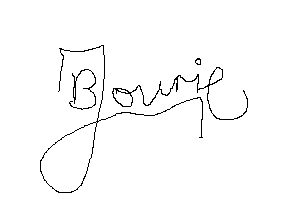
\includegraphics[scale=0.4]{./Figures/Signature.png}\\
\noindent%
\parbox{.5\textwidth}{%
  Signature:\quad\dotfill\par
  \hfill B.\ Fourie\hspace{1.2cm}\null}


\vspace{1.5cm}
\noindent%
\parbox{.5\textwidth}{%
  Date:\quad\dotfill\par}

\tableofcontents
\listoffigures
\listoftables
\chapter{Nomenclature}

\begin{Nomencl}
 \NomGroup{Constants}%-----------------------------------------------
   %\item[$\mathrm{g} = $] $\mathrm{9.81\,m/s^2}$

 \NomGroup{Variables}%-----------------------------------------------
   \item[$P$]
                      \UnitLine{Power}{W}
    \item[$I$]
                      \UnitLine{Current}{A}
    \item[$V$]
                      \UnitLine{Voltage}{V}
    \item[$R$]
                      \UnitLine{Resistance}{\Omega}
    \item[$F$]
                      \UnitLine{Capacitance}{F}
    \item[$H$]
                      \UnitLine{Inductance}{H}
    \item[$f$]
                      \UnitLine{Frequency}{Hz}
    \item[$\eta$]
                      \UnitLine{Efficiency}{\%}
\end{Nomencl}


\endinput


\mainmatter%=========================================================

\chapter{Signal conditioning system design}
\section{System overview} \label{sec:system}
%Here you insert a block diagram of your operational signal conditioning system. There is no need to specify the capacitor and resistor values here, but you want to capture the higher-level functional arrangement you have opted for. The diagram ties together the other chapters in this report and helps the reader understand how you have connected the different funtional blocks together to produce the outputs. For example, a block could be ``Differential aplifier'' or ``level shifting op-amps'' or the like. Fig.\ \ref{fig:system_diagram} as an example that is completely irrelevant and just holds space. 

A system capable of measuring voltages and currents as well as the phase differences between these sinusoidal signals can be seen in Figure \ref{fig:system_diagram}. Load voltage levels were stepped down using a voltage divider before measurements, and the current through the load was measured by amplifying the voltage over a sense resistor. Phase differences were measured by using comparators and a XOR gate to generate a PWM signal, this PWM signal was then scaled to a voltage level by using a simple low pass filter. To keep the design simplistic and the measurement circuitry reliable, only the \SI{5}{\volt} rail was used for this design, with a total expected current draw of \SI{7.2}{\milli A}.

\begin{figure}
    \centering
    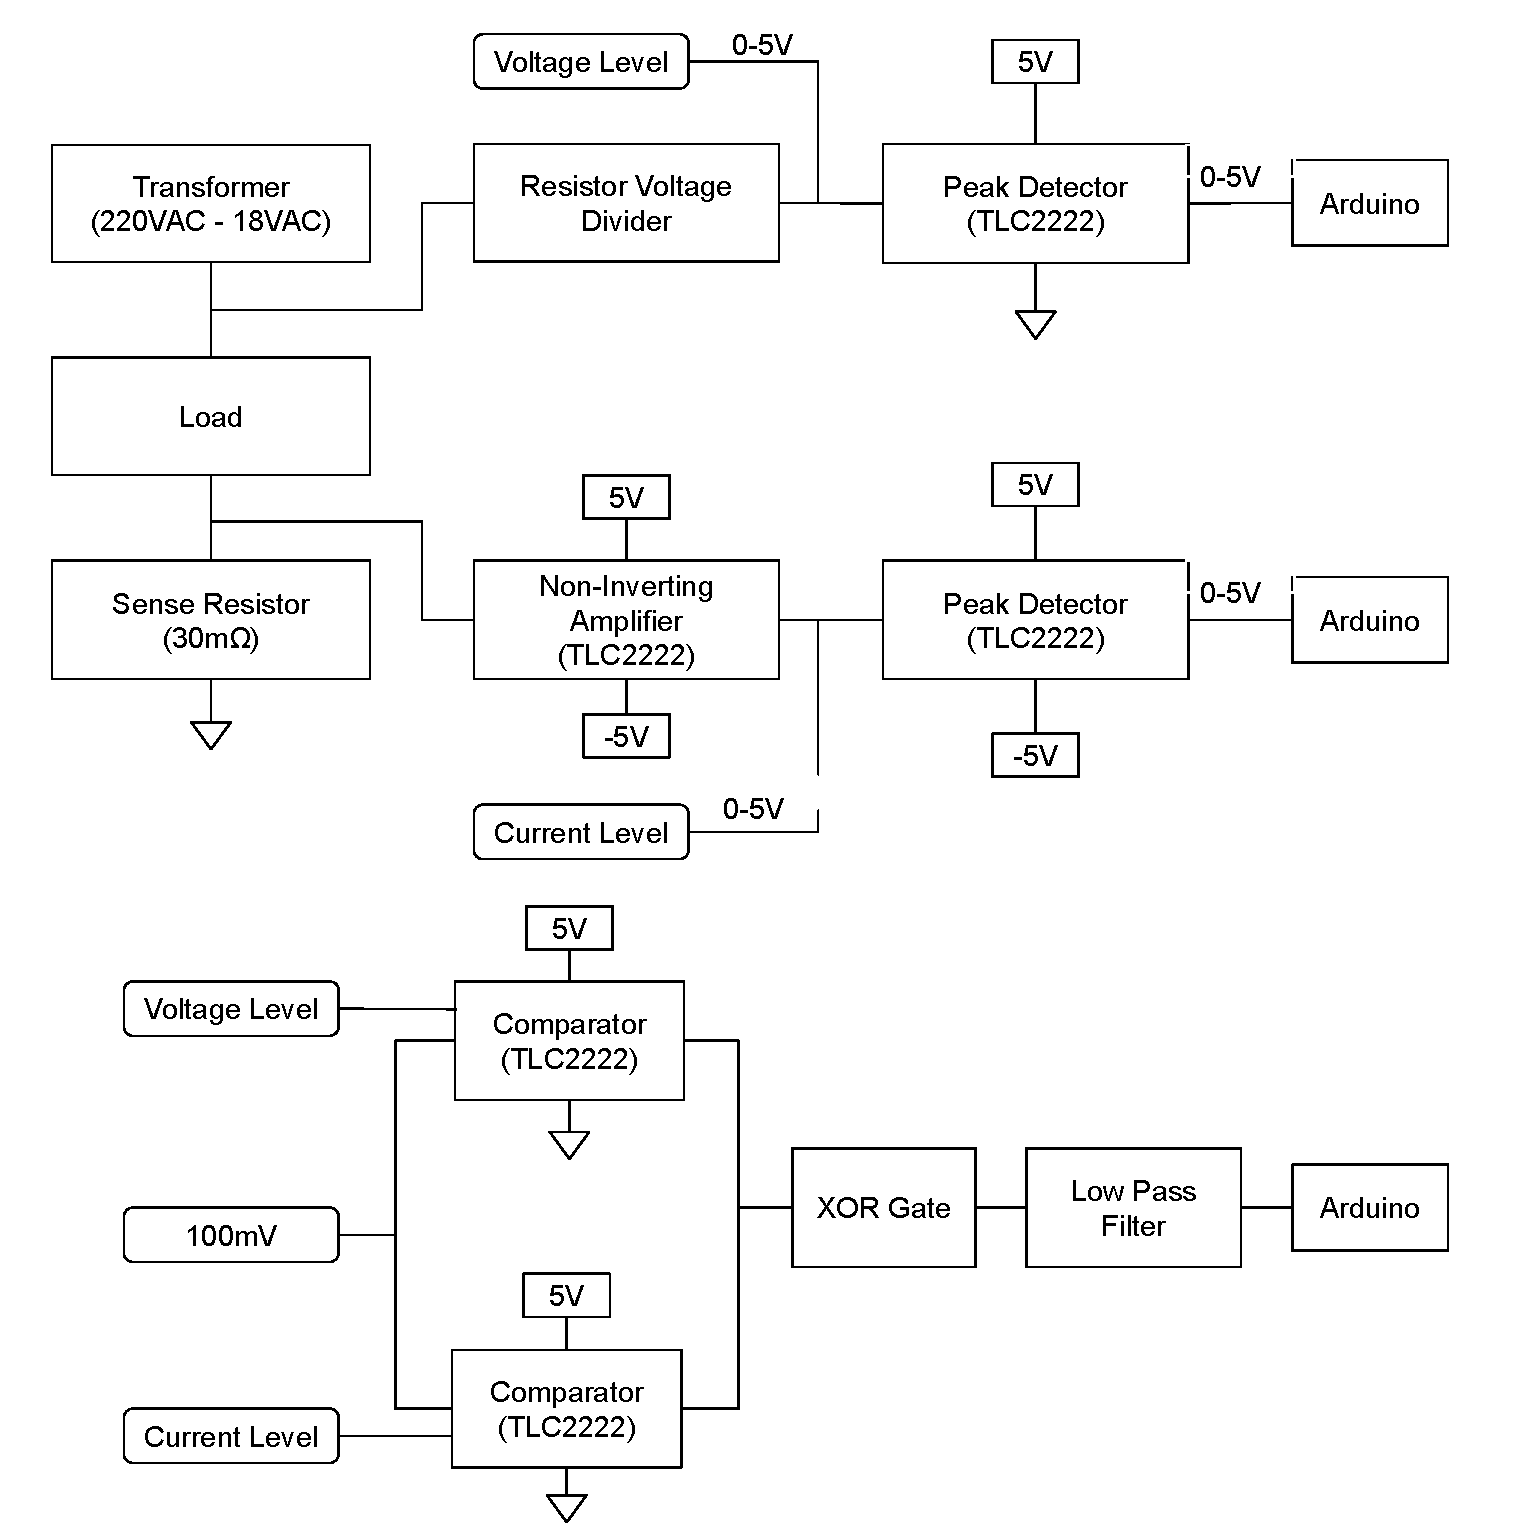
\includegraphics[width = 0.46\linewidth]{Figures/measurement_diagram.pdf}
    \caption{Signal Conditioning Diagram}
    \label{fig:system_diagram}
\end{figure}










\chapter{Power conversion}\label{ch:power_conversion}

The full power supply system with the interaction between all of the different regulation stages is shown Figure \ref{fig:circuit_diagram_power}. A half wave rectifier was chosen as the first stage of the power supply system, this was chosen as it requires less diodes than a full wave rectifier, however a drawback is that a larger smoothing capacitor is required. The second part of this power supply system constitutes a SMPS buck converter implemented to decrease the input voltage to an intermediary voltage usable by the final regulation stages. This buck converter works by charging up an inductor, which stores energy in the form of a magnetic field. If the voltage supplied to the inductor is removed it will reverse the polarity of its voltage and will supply the load with the energy stored in its magnetic field. Through this constant switching between the on and off state the converter is able to decrease the voltage from the input to the output at very high efficiency \cite{Gao:2015}.\vspace{4mm} \newline
The \SI{5}{V} regulator was implemented as a linear regulator, which is a device that uses a closed feedback loop to continuously adjust a voltage divider network to maintain a constant output voltage. The main drawback of this regulation topology is that efficiency is limited as the difference between the input and output voltage is dissipated as heat. Finally the \SI{-5}{V} regulator was implemented as a charge pump, which is a type of switching regulator that delivers power by alternatively charging and discharging capacitors and is specifically useful for supplying circuits with a low load current \cite{WebsiteChargePump}.

\begin{figure}[!ht]
  \centering
 \footnotesize
        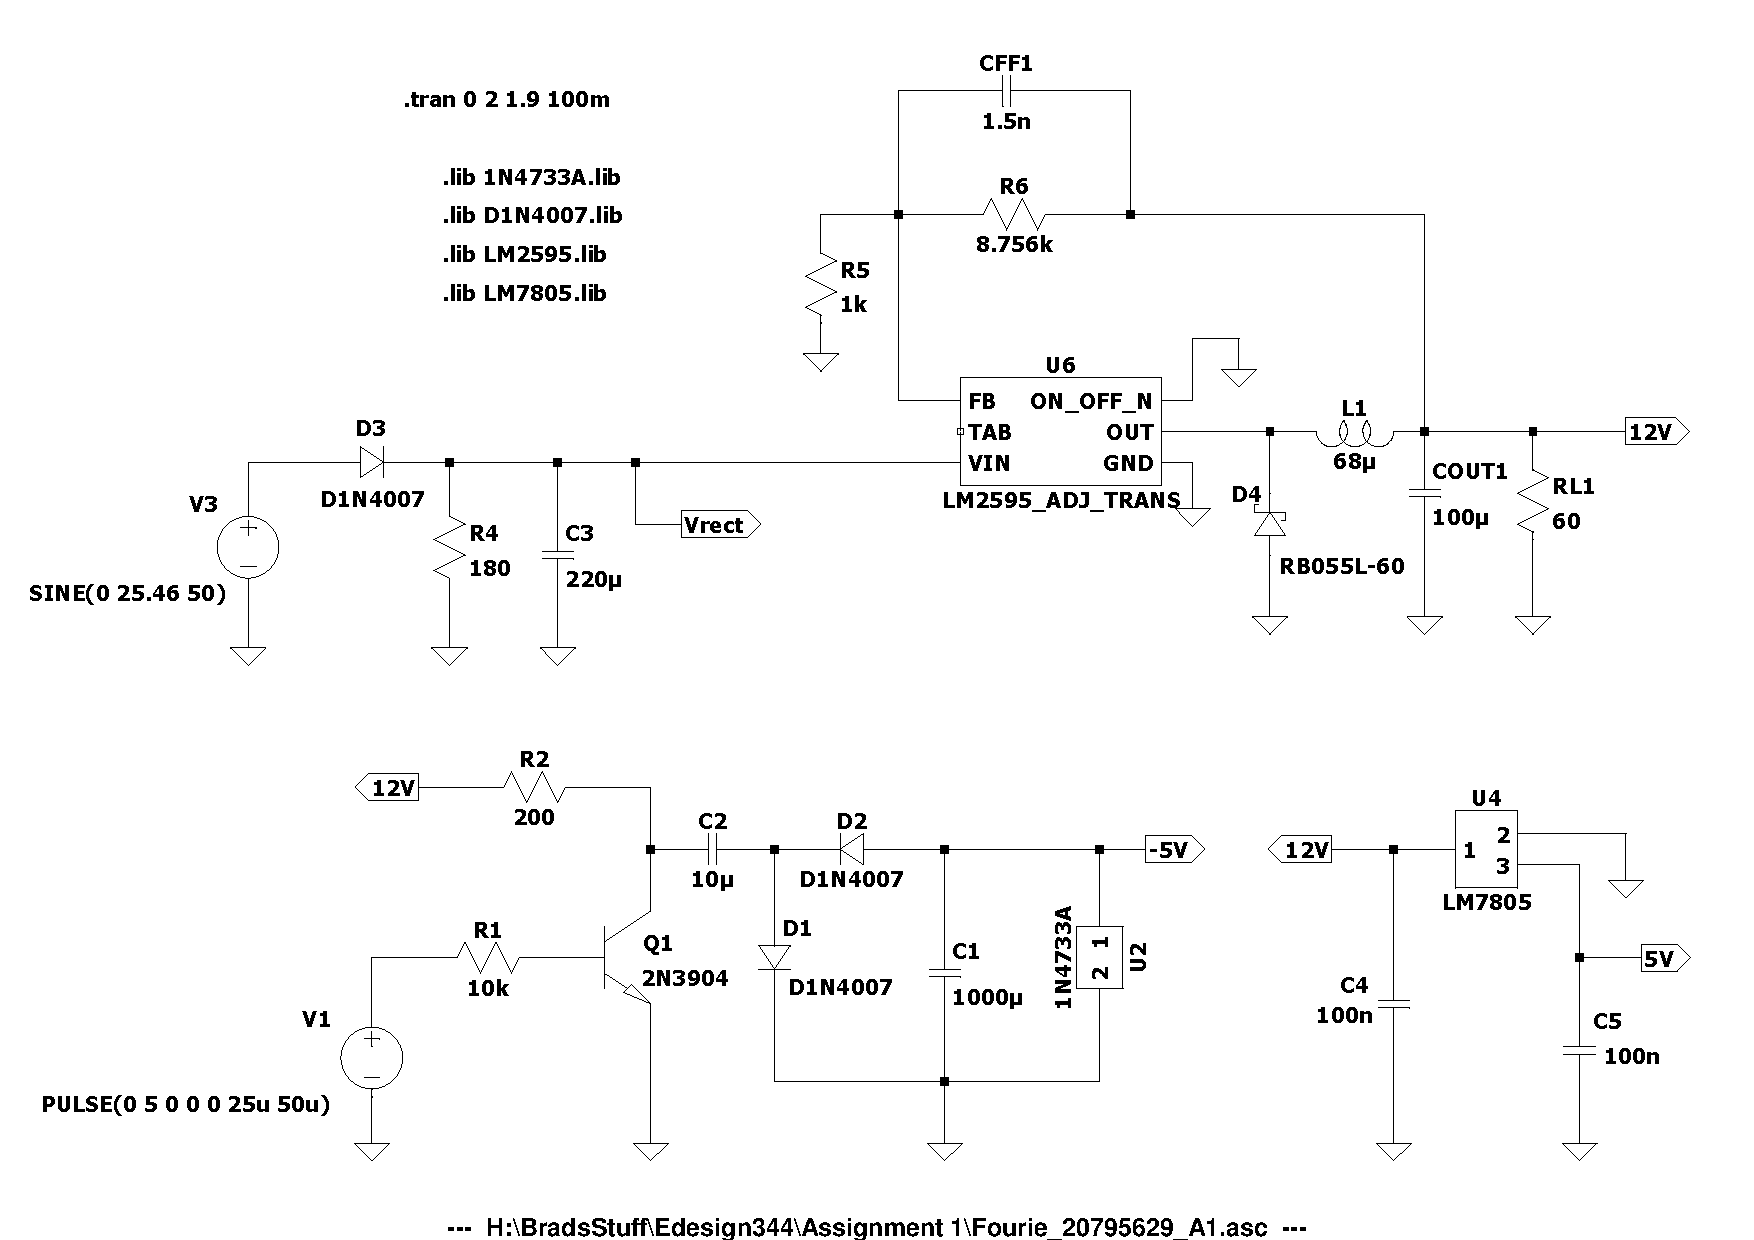
\includegraphics[width=0.75\linewidth]{./Figures/circuit_diagram_power.pdf}
		    \caption{Power conversion circuit diagram.} \label{fig:circuit_diagram_power}
 \end{figure}
%**********************************************
\section{Design} \label{sec:pwr_design}
 
%**********************************************
\subsection{Rectifier}
Firstly a suitable output voltage, allowable output voltage ripple as well as a maximum load requirement had to be chosen. The maximum input voltage was chosen as $\SI{24}{V_{RMS}}$ and a ripple of $50\%$ was chosen, it is worth noting that from \cite{1n4007:2011} the voltage drop over the diode was found as $\SI{1}{V}$ which meant that the output voltage of the rectifier would always be $\SI{1}{V}$ less than the peak value of the sinusoidal input. Referring to the 1N4007 diode datasheet it was confirmed that the full load current draw did not exceed the $\SI{1}{A}$ maximum forward current of the diode. Using Equation \ref{eq:rectifierripple} from \cite{Neaman:2018} the required capacitor was found to be \SI{222.22}{\micro F}, thus a standard \SI{220}{\micro F} was chosen.
\begin{equation}
   V_{r} = \frac{V_{m}}{fRC}
   \label{eq:rectifierripple}. 
\end{equation}

\subsection{Switchmode regulation}
A LM2595 was implemented to control the switching frequency of the switch mode power supply in order to supply an adjustable output of \SI{12}{V}. A series buck regulator in the adjustable output configuration was chosen for the design so that the output could be fine tuned using a potentiometer. The input voltage ranges for the switch mode power supply was chosen as \SI{24.46}{V} to \SI{33.94}{V}, with a maximum supply current chosen as \SI{50}{\milli A}, this was much less than the maximum input voltage of $\SI{45}{V}$ that the regulator is rated for. From the datasheet under these circumstances the regulator operates at roughly $78\%$ efficiency \cite{lm2593:2013}. In order to set the output voltage Equation \ref{eq:smpsresistor} had to be used to choose a ratio of $R_{1}$ to $R_{2}$ to supply the correct output voltage, $R_{1}$ was chosen as $\SI{1}{\kilo \Omega}$, and $V_{ref}$ was given as \SI{1.23}{V}, thus $R_{2}=\SI{8.756}{\kilo \Omega}$. Following this a $\SI{68}{\micro H}$ inductor was chosen following the datasheet. \vspace{4mm} \newline
An output capacitor $C_{out}$ with a low ESR rating, smaller than $\SI{330}{\micro F}$ had to be chosen. A $\SI{100}{\micro F}$ capacitor was chosen, however since this capacitor did not have a low ESR rating a decoupling capacitor had to be placed in parallel with it to remove any ripple voltage due to the high 150kHz switching frequency of the regulator. It is worth noting that this capacitor had to have a voltage rating 1.5 times larger than the 12V output voltage. The same procedure had to be applied for the input bypass capacitor, which was chosen as a $\SI{220}{\micro F}$ capacitor rated for $\SI{50}{V}$ to prevent any large transients from appearing on the input. As an output voltage larger than 10V was chosen for this design a $\SI{1.5}{\nano F}$ ceramic compensation capacitor needed to be added in parallel with $R_{2}$ to provide the necessary stability. Finally a flyback diode $D_1$ had to be added in parallel with the inductor to eliminate any voltage spikes during switching \cite{WebsiteFlyback}. This diode was required to be a fast recovery Schottky diode with a maximum current rating of 1.3 times larger than the load current, and an input voltage 1.25 times larger than the maximum input voltage, for this purpose a 1N5822 was chosen.
\begin{equation}
   V_{out} = V_{ref}(1+\frac{R_{2}}{R_{1}})
   \label{eq:smpsresistor}
\end{equation} 

\subsection{Linear regulation}
A MC78L05 was chosen to supply the $\SI{5}{V}$ rail of the system, since this regulator could handle up to $\SI{35}{V}$ input voltages it was compatible with the maximum $\SI{12}{V}$ output from the intermediary voltage stage. To ensure that the integrated chip could handle the required power requirements the necessary heat sink calculations needed to be completed. \newline 
Given these design requirements a $\SI{7}{V}$ difference was induced across the input and output of the regulator, and a maximum output current of $\SI{40}{\milli A}$ was chosen, which was less than the $\SI{100}{\milli A}$ current the regulator can supply. Furthermore under these conditions a power dissipation of $\SI{280}{\milli W}$ can be expected, which is much less than the $\SI{750}{\milli W}$ maximum power dissipation the regulator is designed for \cite{reg78L05:2002}. By applying Equation \ref{eq:mc78l05temp} from \cite{Perold:2019} and choosing an ambient temperature of $\SI{25}{\degree C}$, the maximum induced temperature was found to be $\SI{67}{\degree C}$, which is far below the maximum allowable operating temperature of $\SI{150}{\degree C}$.\newline
\begin{equation}
   T_{max} = P_{max}(R_{\Theta _{JA}}) + T_{A}
   \label{eq:mc78l05temp}
\end{equation}
An additional capacitor was added to the input of the regulator as to reject attenuation and specifically AC noise from the switchmode regulator. Another capacitor was added to the output of the regulator in order to improve stability and to improve the regulators transient response, both of these capacitors were chosen according to datasheet recommendations.

\subsection{Charge pump regulation}
The first step in designing the charge pump was to select a charge tank capacitor that would ensure a continuous supply of current to the load. For the purpose of this design a $\SI{1}{\milli F}$ capacitor was chosen to supply a maximum of 5mA, and to remove any ripple voltages a $\SI{10}{\nano F}$ capacitor was placed in parallel with it. A secondary smaller capacitor had to be designed to discharge completely within the period of the $\SI{10}{\kilo Hz}$ pulse train to supply charge to the larger capacitor, here a low ESR $\SI{10}{\micro F}$ capacitor was chosen.\vspace{4mm} \newline
A common emitter configuration was chosen to provide a current gain to the output whilst providing no voltage gain, with suitable collector and base resistors designed such that the transistor could turn on and current could flow such as to charge up the capacitor. A base resistor of $\SI{10}{\kilo \Omega}$ was chosen to minimize current losses through the transistor, and a collector resistor of $\SI{200}{\Omega}$ was chosen to supply enough current to the $\SI{-5}{V}$ rail without exceeding the $\SI{625}{\milli W}$ maximum power rating of the transistor.

%**********************************************
\section{Simulation} \label{sec:pwr_simu}
%**********************************************
The rectifier circuit was simulated with a $\SI{18}{V_{RMS}}$ input, with this maximum voltage ripple shown in Figure \ref{subfig:pwr_simu_rect}. For this nominal supply input a ripple of only $34.8\%$ was reported, which was below the maximum ripple designed for. The complete power regulation system was simulated as to obtain the steady state DC voltage values of the rails, Figure \ref{subfig:pwr_simu_rails_pos} displays the output of the $\SI{5}{V}$ regulator and Figure \ref{subfig:pwr_simu_rails_neg} displays the output of the $\SI{-5}{V}$ regulator, from this we can confirm that by simulation the power supply system was designed correctly.

%**********************************************
\section{Measurements} \label{sec:pwr_meas}
%**********************************************
The power system as a whole was tested with the rail voltages supplied by the charge pump and linear regulators respectively, which in turn were powered by the intermediary voltage stage which received its input from the rectified transformer output. The measured output voltage of the linear regulator was found to be $\SI{5.12}{V}$ under full load conditions supplying $\SI{40}{\milli A}$ as shown in Figure \ref{subfig:pwr_meas_rails_pos}, under these circumstances the efficiency of the regulator was calculated as $37.3\%$ using Equation \ref{eq:efficiency} at a maximum quiescent current of $\SI{5.5}{\milli A}$. As can be seen in Figure \ref{subfig:pwr_meas_noise_pos} a noise level of less than $\SI{10}{\milli V}$ peak to peak was measured on the $\SI{5}{V}$ rail, which confirms that the regulator met all the required specifications.
\begin{equation}
   \eta = \frac{P_{out}}{P_{in}}
   \label{eq:efficiency}
\end{equation}
The charge pump supplied a stable $\SI{-5.12}{V}$ output under no load conditions as can be seen in Figure \ref{subfig:pwr_meas_rails_neg}, with noise not exceeding $\SI{9.28}{\milli V}$ peak to peak as can be seen in Sub figure \ref{subfig:pwr_meas_noise_neg}. After a $\SI{10}{\kilo \Omega}$ load was applied to regulator, it was found that the output voltage level dropped to $\SI{-4.76}{V}$.

\section{Summary and implementation}
The power regulation system implemented for this system met all of the design requirements and can be seen in Figure \ref{subfig:pwr_pcb}. The rectification stage of the power supply which rectified the transformer supply voltage had a ripple voltage of less than 35\%, and could successfully supply the input voltage and current required for the intermediary switchmode power supply stage. This buck converter output a stable $\SI{12}{V}$ output and successfully supplied the inputs to both the charge pump and linear regulator. The linear regulator supplying the $\SI{5}{V}$ rail operated successfully under full load conditions and could supply a steady output under all required loading conditions, however the charge pump supplying the $\SI{-5}{V}$ rail could not supply enough current for the purpose of this design, therefore it was decided that it would not be used to supply the signal conditioning circuitry.

\begin{figure}[!ht]
    \centering
  	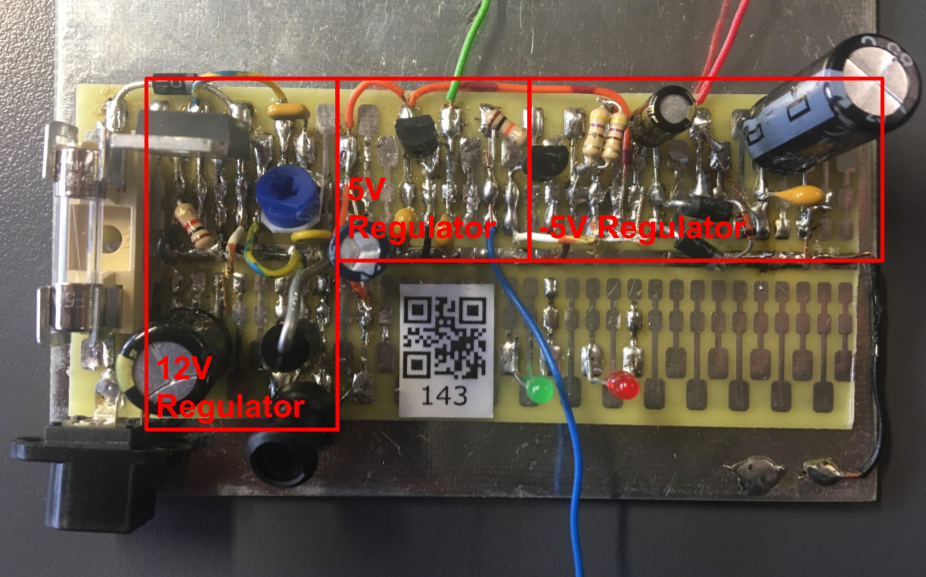
\includegraphics[width=0.5\linewidth]{./Figures/pwr_pcb.png}
	\caption{Implementation of the power conversion circuitry. } \label{subfig:pwr_pcb}
\end{figure}

\begin{figure}
 \footnotesize
 \centering
    \begin{subfigure}[]{0.35\textwidth}
              \centering
  		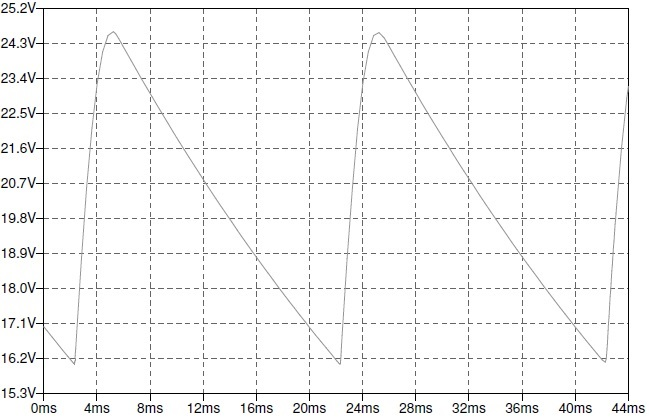
\includegraphics[width=1\linewidth]{./Figures/pwr_simu_rect.JPG}
		    \caption{} \label{subfig:pwr_simu_rect}
     \end{subfigure}
          \begin{subfigure}[]{0.35\textwidth}
             \centering
  		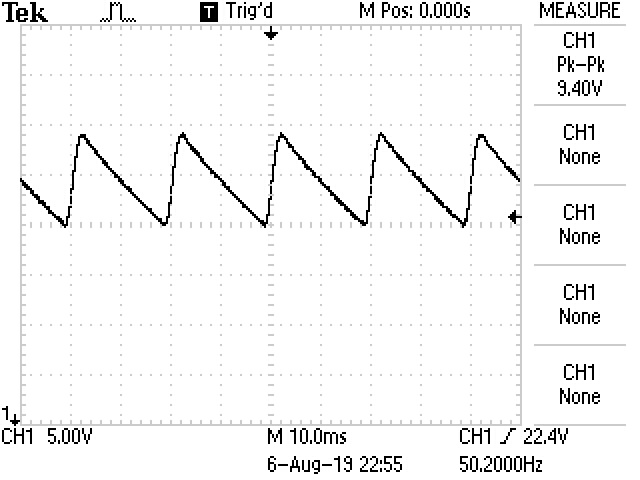
\includegraphics[width=1.0\linewidth]{./Figures/pwr_meas_rect.jpg}
		   \caption{ } \label{subfig:pwr_meas_rect}
     \end{subfigure}
    \begin{subfigure}[]{0.35\textwidth}
              \centering
  		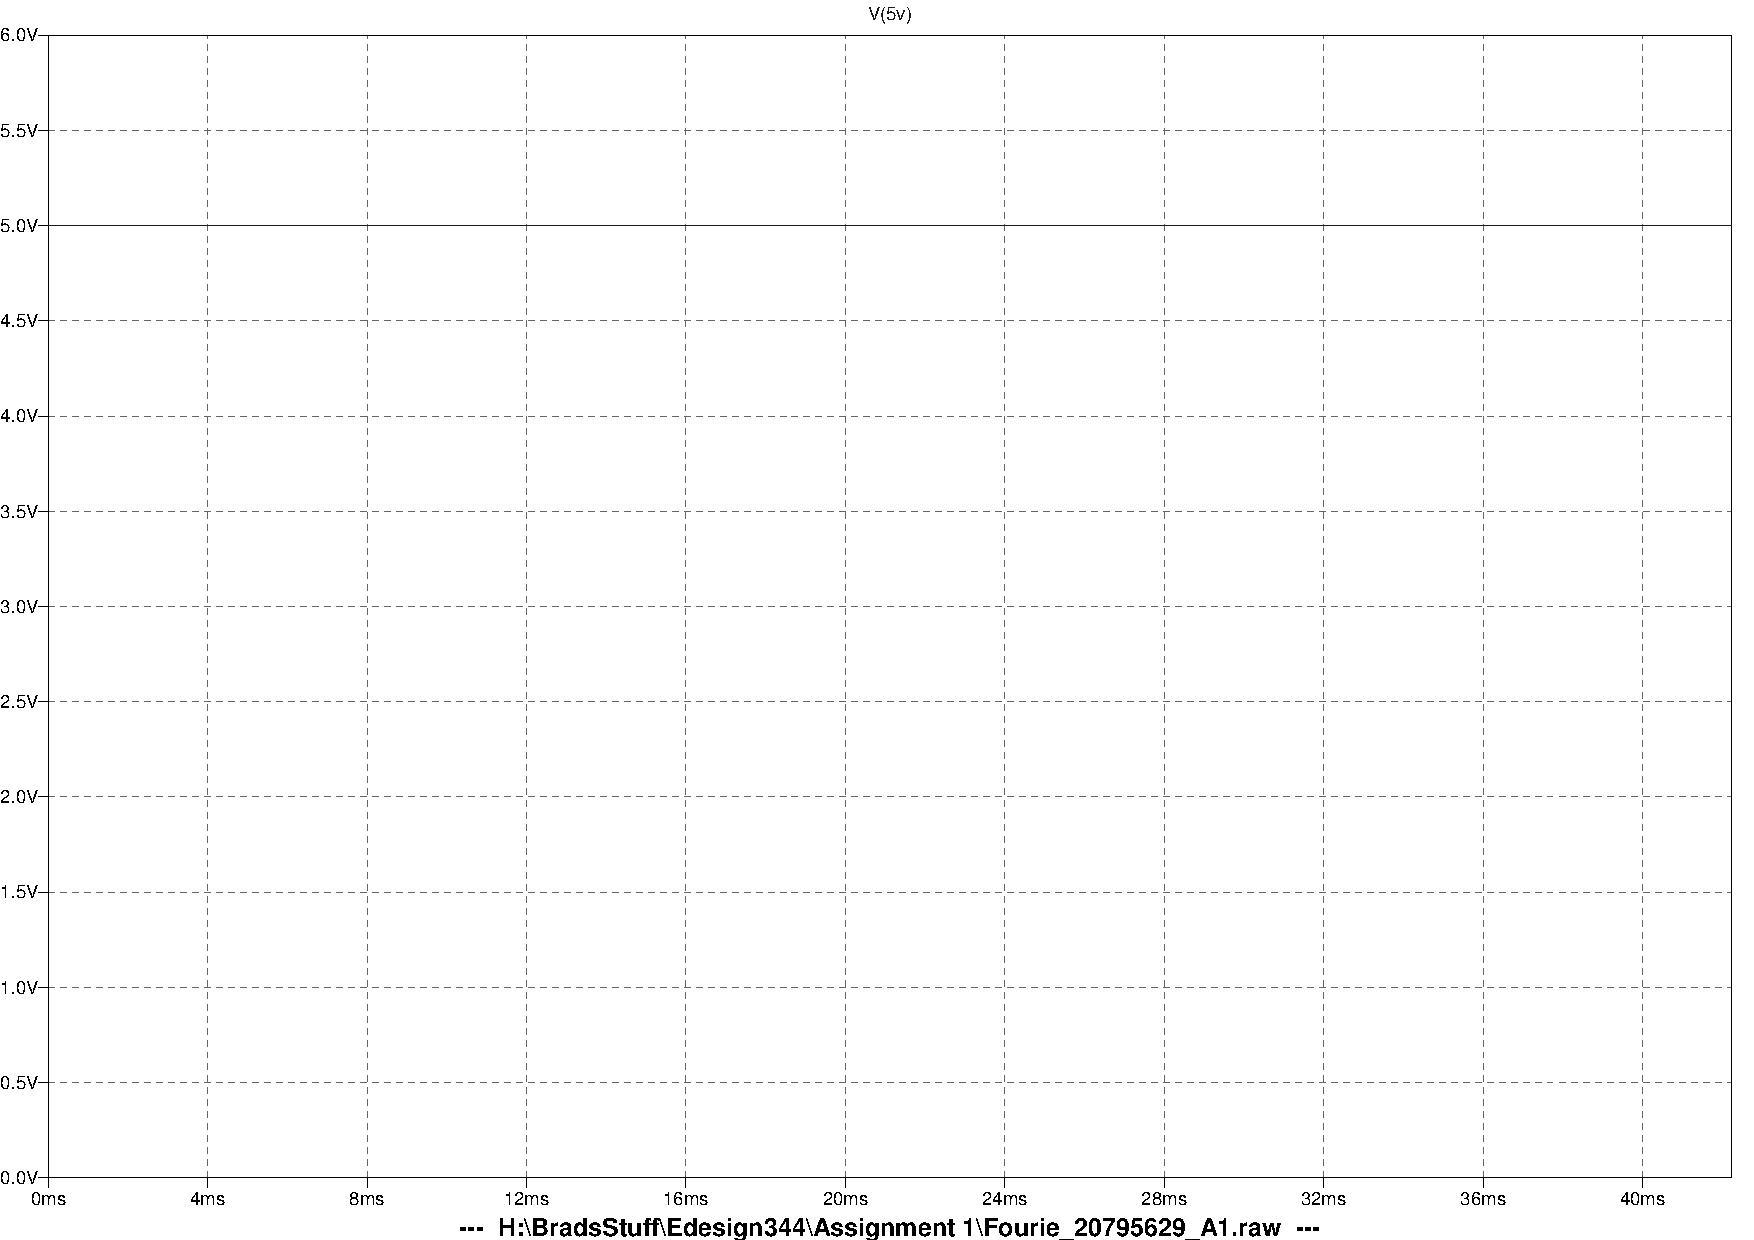
\includegraphics[width=1\linewidth]{./Figures/pwr_simu_rails_pos.pdf}
		    \caption{} \label{subfig:pwr_simu_rails_pos}
     \end{subfigure}
    \begin{subfigure}[]{0.35\textwidth}
              \centering
  		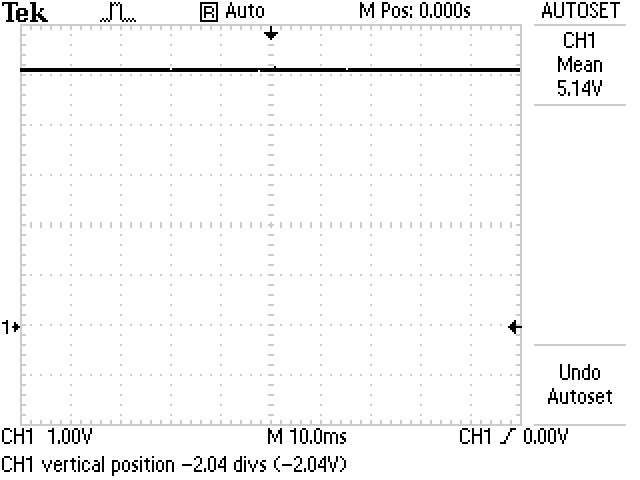
\includegraphics[width=1\linewidth]{./Figures/pwr_meas_rails_pos.JPG}
		    \caption{} \label{subfig:pwr_meas_rails_pos}
     \end{subfigure}
    \begin{subfigure}[]{0.35\textwidth}
             \centering
      		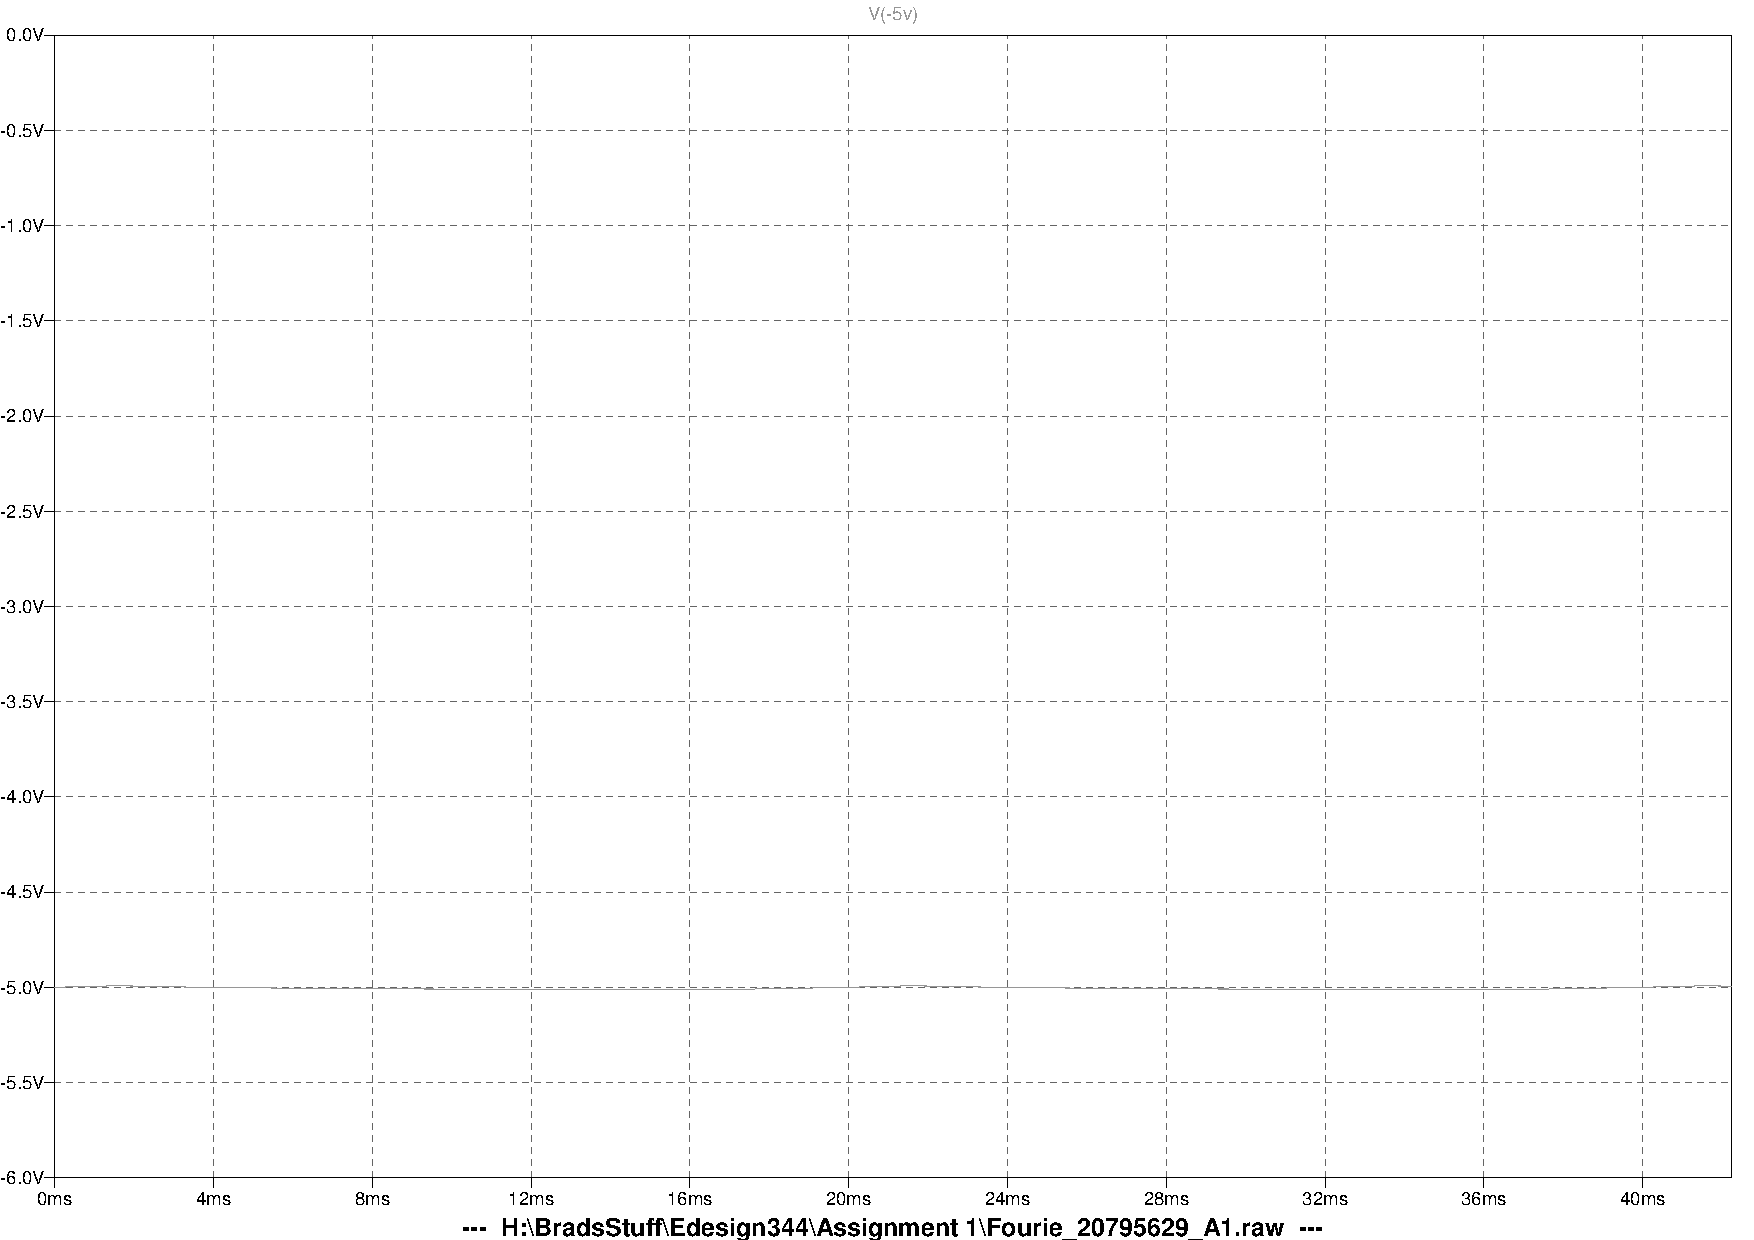
\includegraphics[width=1.0\linewidth]{./Figures/pwr_simu_rails_neg.pdf}
		   \caption{ } \label{subfig:pwr_simu_rails_neg}
     \end{subfigure}
    \begin{subfigure}[]{0.35\textwidth}
             \centering
  		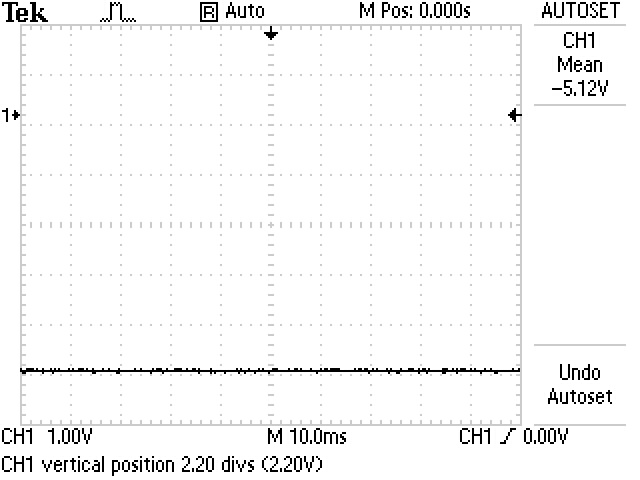
\includegraphics[width=1.0\linewidth]{./Figures/pwr_meas_rails_neg.JPG}
		   \caption{ } \label{subfig:pwr_meas_rails_neg}
     \end{subfigure}
    \begin{subfigure}[]{0.35\textwidth}
              \centering
  		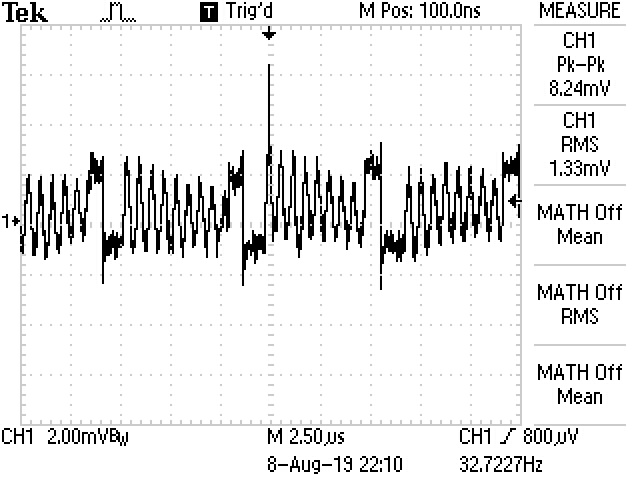
\includegraphics[width=1\linewidth]{./Figures/pwr_meas_noise_pos.JPG}
		    \caption{} \label{subfig:pwr_meas_noise_pos}
     \end{subfigure}
    \begin{subfigure}[]{0.35\textwidth}
             \centering
  		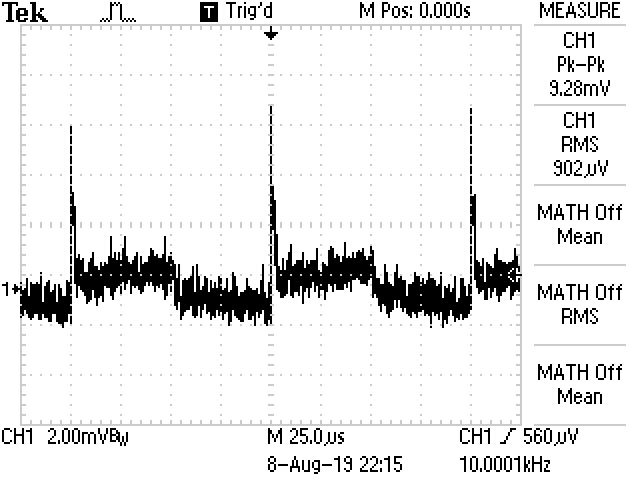
\includegraphics[width=1.0\linewidth]{./Figures/pwr_meas_noise_neg.JPG}
		   \caption{ } \label{subfig:pwr_meas_noise_neg}
     \end{subfigure}
   \caption[Measured regulated output voltage plots]{Power conditioning: (a) Simulation of the rectification showing the rectified signal. (b)  Measurement of the rectification showing the rectified signal.  (c)  Simulation output of the positive voltage rail level. (d) Measurement of the positive voltage rail level. (e)  Simulation output of the negative voltage rail level. (g) Measurement of the negative voltage rail level. (g)  Measurement of the noise on the postive voltage rail. (h) Measurement of the noise on the negative voltage rail. }
    \label{fig:simulation_results_box}
 \end{figure}


\chapter{Current peak transducer}
\section{Theory and related work} \label{sec:literature_current_peak_transducer}
The design for the current peak transducer consisted of a current sense resistor in series with the load, a non inverting operational amplifier gain stage, and a precision rectifier implemented as in Section \ref{sec:design_voltage_peak_transducer}. A current sense resistor is a resistor placed in series with a load to allow current to be measured, the voltage across the resistor will be directly proportional to the current being measured. A non inverting amplifier is an operational amplifier configuration where the input voltage signal is connected to the non-inverting input to the operational amplifier. The feedback control consists of a resistor divider network that connects the output to the inverting input, this resistor divider network sets the gain of the amplifier, produces a good stability and has a high input impedance \ref{yourmom}. 
%https://www.electronics-tutorials.ws/opamp/opamp_3.html

\section{Design} \label{sec:design_current_peak_transducer}
The first part of this design included a sense resistor which was added in series with the load to turn a current measurement into a voltage measurement, this voltage measurement was then amplified to a suitable voltage level usable by the peak transducer. For the purpose of this design a $\SI{30}{\milli \Omega}$ sense resistor was chosen to ensure a reasonable trade off between power losses in the system and the measured voltage level over the sense resistor. It was found that a smaller sense resistor would by Ohm's law have a smaller voltage drop over it, and this in return would require a larger voltage gain stage, which was not desirable as such a large gain would require a very large feedback resistor, with a very large deviation from its given resistance. It was chosen that the current peak transducer would be able to measure a maximum current of \SI{350}{\milli A}, this corresponded to a sense voltage of \SI{10.5}{\milli V}.\newline
The Arduino's maximum pin voltage was given as \SI{5}{\volt}, and to ensure a maximum resolution for the \SI{350}{\milli A} measurement range, the \SI{10.5}{\milli V} maximum sense voltage had to be amplified using an operational amplifier. This operational amplifier configuration was chosen as a differential mode non-inverting amplifier utilizing only the SI{5}{\volt} and rail as its power supply. It was found that the maximum input to any of the operational amplifiers pins was not to exceed \SI{5}{\volt} or \SI{-0.3}{\volt} \ref{yourmom}.
The desired gain, and ratio between input resistor $R_1$, and feedback resistor $R_2$ was calculated by using Equation \ref{eq:opampgain}. Here $R_1$ was chosen as $\SI{1}{\kilo \Omega}$, and given this $R_2$ was found to be $\SI{470}{\kilo \Omega}$.\newline
\begin{equation}
   \frac{V_{out}}{V_{in}}=1+\frac{R_2}{R_1} 
   \label{eq:opampgain}
\end{equation}
Given that the sense voltage was now amplified to a suitable range between 0 and \SI{5}{\volt} the same design procedure as Section \ref{sec:design_voltage_peak_transducer} could be applied to measure the amplitude of the peak of the sinusoidal input. A ripple voltage of no more than \SI{5}{\milli \volt} was chosen and from this the output capacitor to the peak detector was calculated in exactly the same way as in Section \ref{sec:design_voltage_peak_transducer} using Equation \ref{eq:ripplevoltage}, the desired capacitor value was found as $\SI{20}{\micro F}$. To minimise the effect of noise on the output of the transducer the smoothing capacitor at the output was chosen as two \SI{10}{\micro F} low ESR capacitors placed in parallel. Decoupling capacitors were also placed at the positive rail of the TLC2272 to keep the effects of the rail voltage noise from the power supply to a minimum on the output.
Given the specification of a maximum load current of \SI{350}{\milli A} corresponding to a voltage of $\SI{5}{VAC}$ and the Arduino having a range of $4095$ bits, it can be calculated that the resolution of the ADC would be $\SI{85.47}{\micro A}$ per bit.
\begin{figure}[h!]
    \centering
    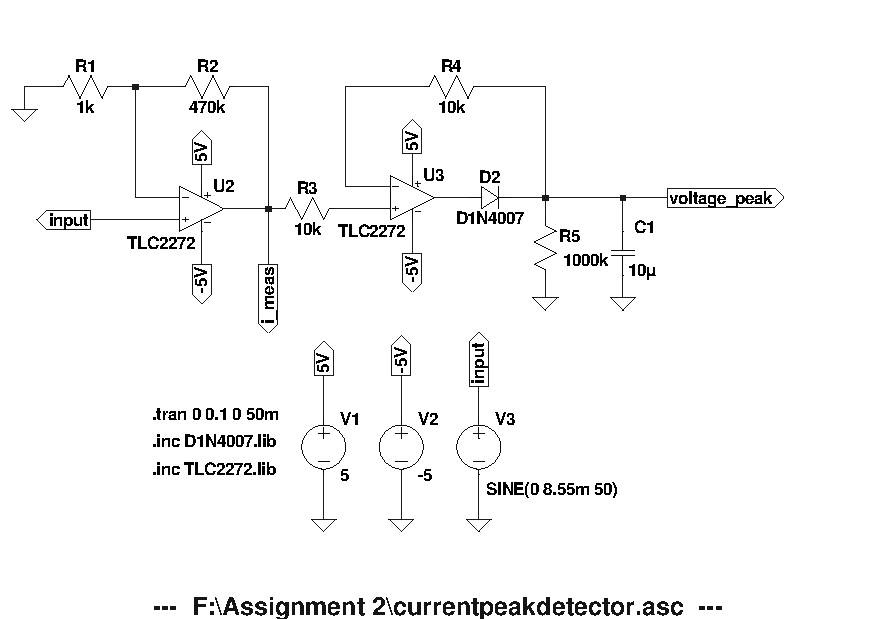
\includegraphics[width = 0.57\linewidth]{Figures/currentpeakdetector.pdf}
        \caption{Current Peak Transducer Diagram}
    \label{fig:currentpeakdetector.pdf}
\end{figure}

\section{Simulation} \label{sec:simulation_current_peak_transducer}
To confirm that the current peak transducer was designed correctly the designed circuit was supplied with a nominal input voltage of \SI{3}{\milli \volt}, this corresponded to a \SI{100}{\milli A} current through the sense resistor, this output can be seen in Figure \ref{subfig:currenttransducer100maripple}. From the output plot we can see that the ripple voltage was simulated to be \SI{9.2}{\milli \volt}, this was slightly higher than what was designed for in the design section, however for this purpose of this design the ripple voltage is acceptable as it does not interfere with the accuracy requirements of the current peak transducer measurement.\vspace{4mm} \newline 
To ensure that the current peak transducer responded to a \SI{10}{\milli A} change in input, for inputs over \SI{100}{\milli A}, within 1 second a \SI{3}{\milli \volt} input was applied and decreased by \SI{300}{\micro \volt}, this change in input voltage corresponded to a decrease in load current by \SI{10}{\milli A}. The result of this simulation can be seen in Figure \ref{subfig:currenttransducerinputchange}, and from this graph we can see that the input responded to the change in input in exactly 1 second. 

\begin{figure}[h!]
 \centering
     \begin{subfigure}[]{0.45\textwidth}
        \centering
         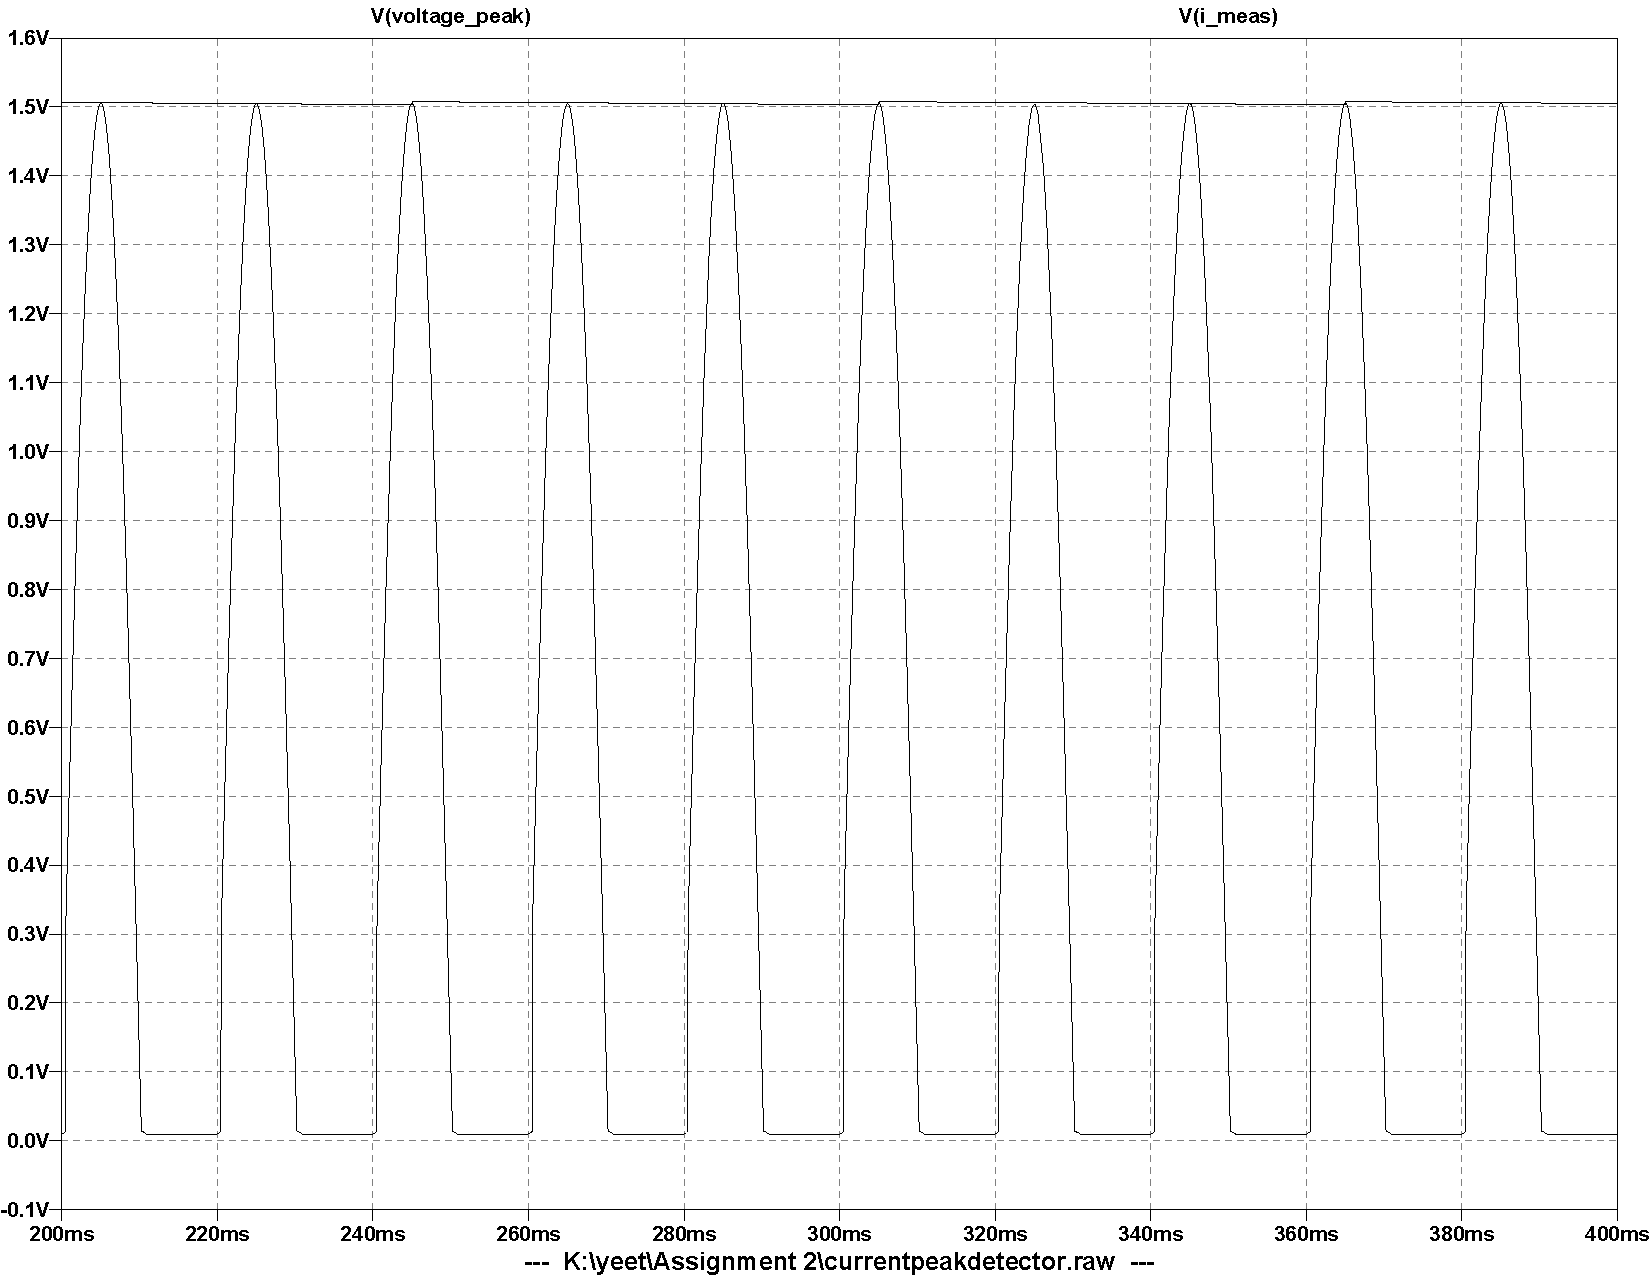
\includegraphics[width=1\linewidth]{./Figures/currentpeakdetectoroutputsim.pdf}
		    \caption{Peak detection of a amplified 100mA input} \label{subfig:currenttransducer100maripple}
     \end{subfigure}
      \begin{subfigure}[]{0.45\textwidth}
              \centering
  		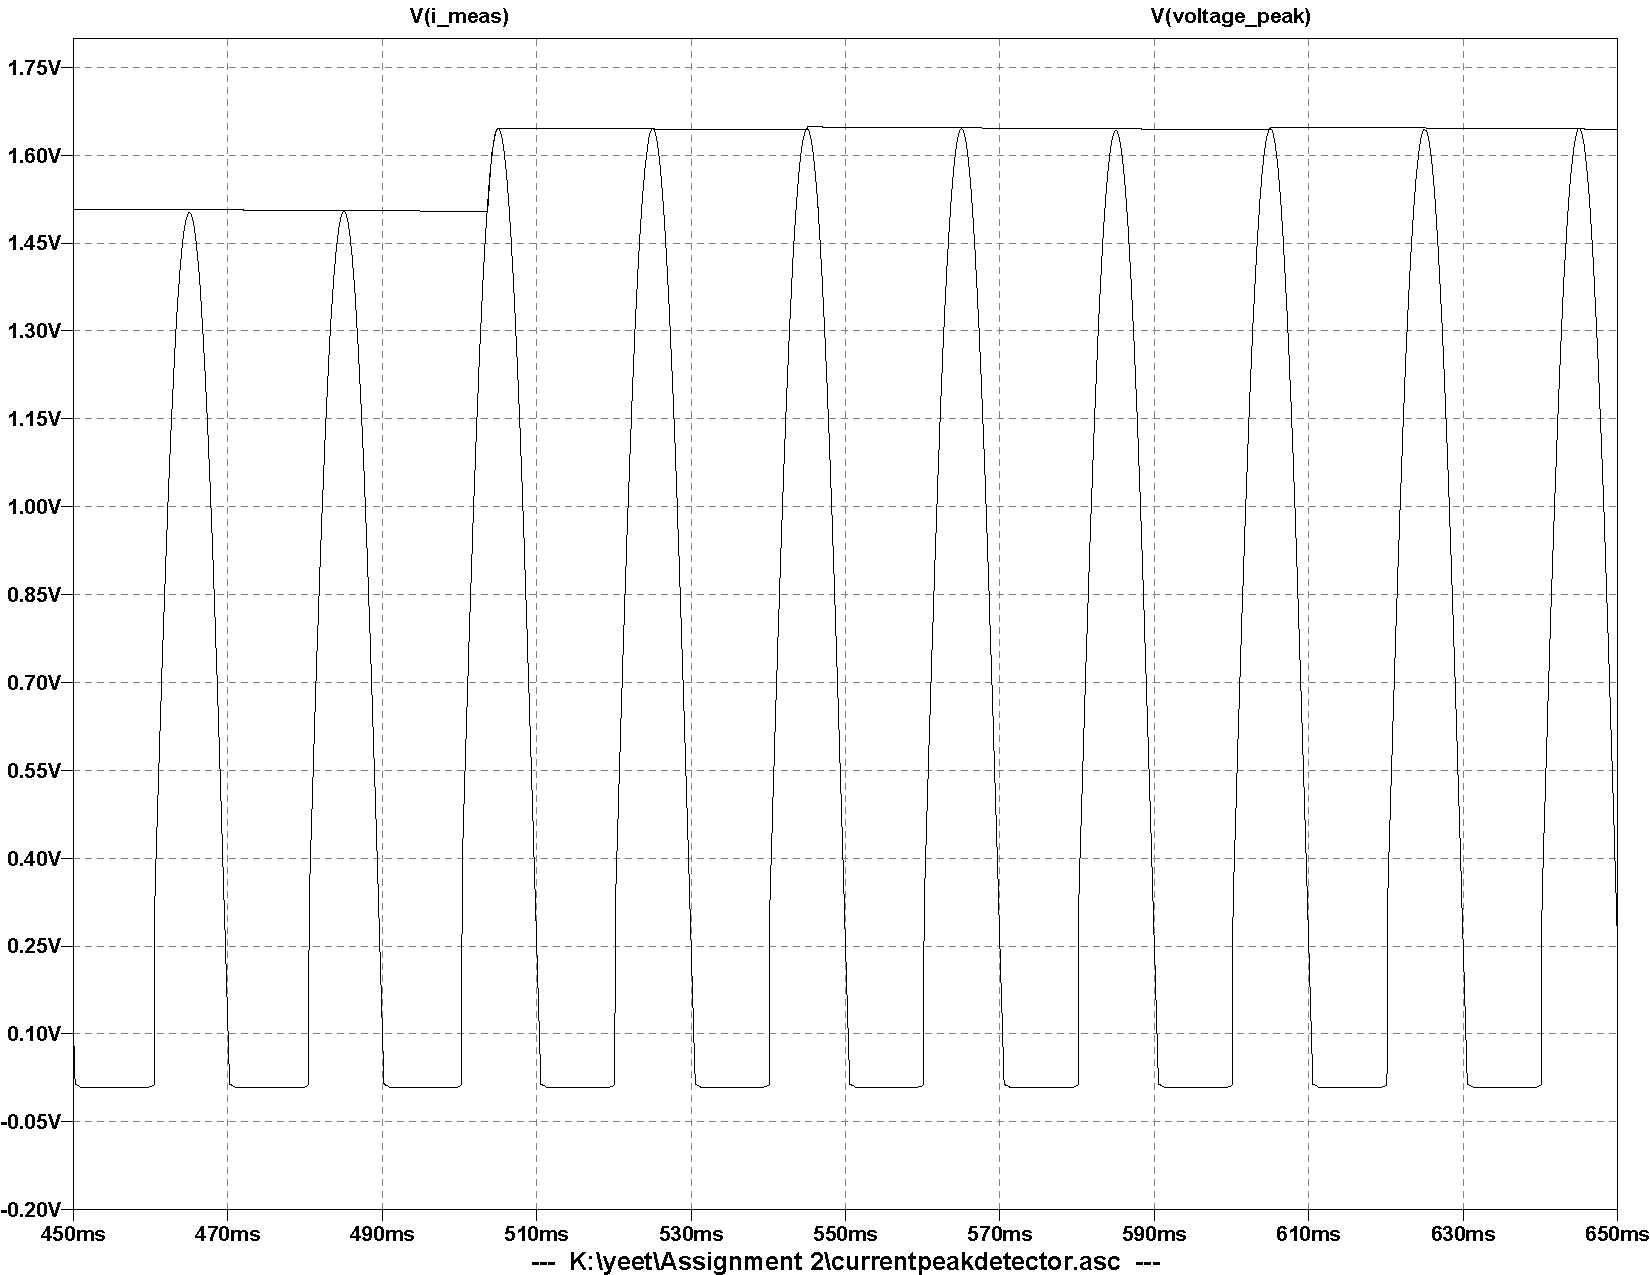
\includegraphics[width=1\linewidth]{./Figures/currentpeakdetectoroutputchange.pdf}
		    \caption{Response given \SI{10}{mA} change in \SI{100}{mA} input} \label{subfig:currenttransducerinputchange}
     \end{subfigure}
   \caption[Simulated results for the current transducer]{Output voltage ripple and response for the current transducer. (a) depicts output voltage ripple, (b) depicts response to change in input current. }
    \label{fig:simulation_results_box}
 \end{figure}


\section{Measurements} \label{sec:measurements_current_peak_transducer}
In order to test the accuracy and precision of the current peak transducer unit tests were performed using an oscilloscope and voltage divider. Since the oscilloscope could not output the small voltages required for the unit tests a voltage divider that divided the oscilloscope output down by a factor of 100 was required in order to obtain the sense voltages in the milli-Volt range. The input current was related to the output voltage by using Equation \ref{eq:currentcalc}. The gain of the operational amplifier gain stage was calculated to be $A_{v}=474.4$ using Equation \ref{eq:opampgain}, and the resistor values for this formula were measured using a multimeter.
\begin{align}
   V_{out}=R_{sense}I_{load}A_{v} \\
   V_{out}= 14.232I_{load} \nonumber
   \label{eq:currentcalc}
\end{align}
The second column in Table \ref{tab:currenttransducerunittests} shows the output as shown on the oscilloscope screen, and the third column shows the measurement found by measuring this output using an oscilloscope. This third column was the input to the voltage circuit, with the actual sense voltage being measured as these values divided by 100. All unit tests were found to be accurate within a maximum difference of only \SI{0.74}{\milli A}, confirming that the design met the requirements. \vspace{4mm} \newline 
The current peak transducer was then testing under real measurement conditions using various load resistors, these results are tabulated in Table \ref{tab:currenttransducerrealtests}, here it was found that all measurements except the no load test was within the \SI{1}{\milli A} design specification. This contradicts the result of the no load measurement difference shown in Table \ref{tab:currenttransducerunittests}, however this difference can be explained by the fact that the input to the operational amplifier was grounded by the signal generator for the unit test, and left floating for the real no load test. \vspace{4mm} \newline  
Figure \ref{subfig:currenttransducermidrange} shows the output of the current peak transducer given a load of  $\SI{1}{\kilo \Omega}$, from the oscilloscope measurements we can see that the difference between the signals is only $\SI{4}{\milli V}$, which by using Equation \ref{eq:currentcalc} is only out by $\SI{0.281}{\milli A}$. The signal quality of the transducer output is shown in Figure \ref{subfig:currenttransducermidrangenoise}, which has a peak to peak range of only $\SI{15.6}{\milli V}$. Due to the fact that the current peak transducer measurements were all within $\SI{1}{\milli A}$ of the actual measurement it was decided that no curve of best fit would be necessary to improve the output of this design.

\begin{table}[h]
        \centering
        \scriptsize
        \caption{Current transducer intermediate unit test results.}
             \begin{tabular}{C{2cm} C{2cm} C{2cm} C{2cm} C{2cm} C{2cm}}
           Emulated level & Signal generator & Signal generator & Analogue output & Deduced input & Difference \\
           ($mA_{peak}$)   & ($mV_{peak}$) & ($mV_{peak}$) & ($VDC$)         & ($mA_{peak}$) & ($mA_{peak}$) \\
           \hline
            0       & 0 & 0 & 0.004 & 0.281 & 0.28\\
            50      & 153.15 & 155.69 & 0.704 & 49.46   & 0.53\\
            100     & 309.12 & 311.32 & 1.416 & 99.49   & 0.51\\
            101     & 311.15 & 314.50 & 1.448 & 101.74  & 0.74\\
            102     & 316.60 & 317.61 & 1.456 & 102.30  & 0.30\\
            200     & 617.00 & 622.77 & 2.846 & 199.97  & 0.03\\
            285     & 879.50  & 887.20 & 4.064 & 285.55  & 0.55\\
          \hline
        \end{tabular}
     \label{tab:currenttransducerunittests}
\end{table}

\begin{table} [h]
        \centering
        \scriptsize
        \caption{Current transducer integrated test results.}
         \begin{tabular}{C{1.4cm} C{1.2cm} C{1.2cm} | C{1.8cm} C{1.8cm} C{2.2cm} C{2cm} C{1.8cm}}
           Measure- & Load $R_1$ & Load $R_2$ & Measured $V_R$ & Actual input & Analogue output & Deduced input & Difference\\
           ment & ($\Omega$) & ($\Omega$) & ($mV_{peak}$) & ($mV_{peak}$) & ($mV_{peak}$) & ($mA_{peak}$) & ($mA_{peak}$) \\
        \hline
            No load      & open & -   & 0      & 0      & 30.8  & 2.164   & 2.16\\
            Full load    & 100  & -   & 9.045       & 301.51 & 4.28  & 300.73  & 0.78\\
            Mid range    & 1k   & -   & 0.906       & 30.159 & 417.6 & 29.40 & 0.76 \\
            Mid + $\delta$    & 1k   & 24k  & 0.943 & 31.415 & 435.4 & 30.59 & 0.69 \\
          \hline
        \end{tabular}
     \label{tab:currenttransducerrealtests}
\end{table}

\begin{figure}[h]
 \centering
     \begin{subfigure}[]{0.45\textwidth}
        \centering
         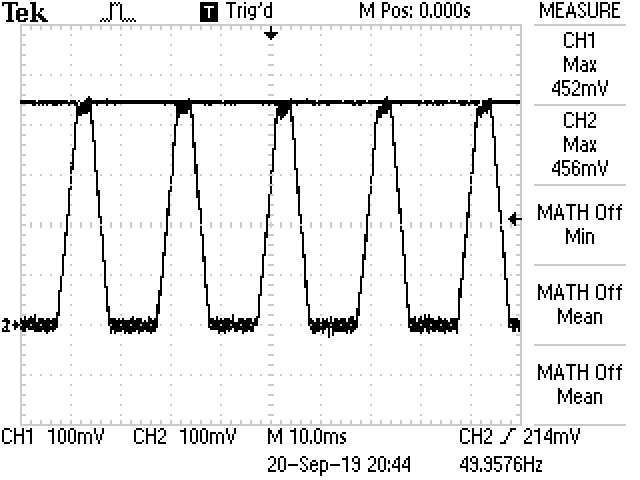
\includegraphics[width=1\linewidth]{./Figures/currenttransducermidrange.JPG}
		    \caption{Mid range measurement result} \label{subfig:currenttransducermidrange}
     \end{subfigure}
      \begin{subfigure}[]{0.45\textwidth}
              \centering
  		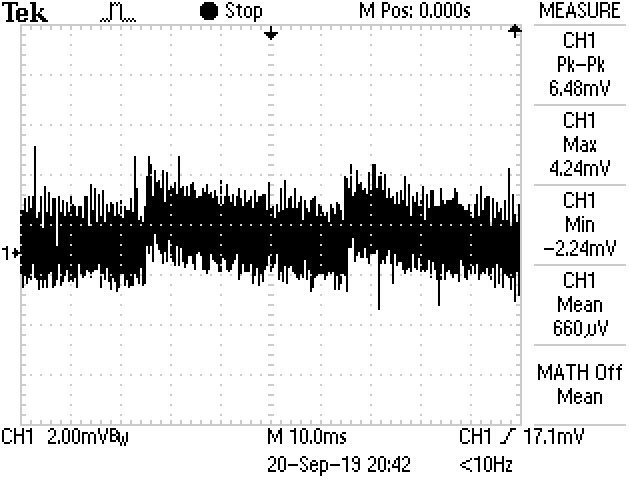
\includegraphics[width=1\linewidth]{./Figures/currenttransducernoise.JPG}
		    \caption{Noise response} \label{subfig:currenttransducermidrangenoise}
     \end{subfigure}
   \caption[Measured results for the current transducer]{Output voltage ripple and response for the current transducer. (a) depicts mid range output, (b) depicts noise response. }
    \label{fig:simulation_results_box}
 \end{figure}






\chapter{Linear regulation}
\section{Theory and related work} \label{sec:literature_linear}
A linear regulator is a device that uses a closed feedback loop to continuously adjust a voltage divider network to maintain a constant output voltage. The main drawback of this regulation topology is that efficiency is limited as the difference between the input and output voltage is dissipated as heat.

\section{Design} \label{sec:design_linear}
For the purpose of this design a MC78L05 was chosen, since this regulator could handle up to $\SI{35}{V}$ input voltages it was compatible with the maximum $\SI{12}{V}$ output from the intermediary voltage stage. To ensure that the integrated chip could handle the required power requirements the necessary heat sink calculations needed to be completed. \newline 
Given these design requirements a $\SI{7}{V}$ difference was induced across the input and output of the regulator, and a maximum output current of $\SI{40}{\milli A}$ was chosen, which was less than the $\SI{100}{\milli A}$ current the regulator can supply. Furthermore under these conditions a power dissipation of $\SI{280}{\milli W}$ can be expected, which is much less than the $\SI{750}{\milli W}$ maximum power dissipation the regulator is designed for \cite{reg78L05:2002}. By applying Equation \ref{eq:mc78l05temp} from \cite{Perold:2019} and choosing an ambient temperature of $\SI{25}{\degree C}$, the maximum induced temperature was found to be $\SI{67}{\degree C}$, which is far below the maximum allowable operating temperature of $\SI{150}{\degree C}$.\newline
\begin{equation}
   T_{max} = P_{max}(R_{\Theta _{JA}}) + T_{A}
   \label{eq:mc78l05temp}
\end{equation}
Referring to Figure \ref{fig:5vregulator} the capacitor C1 had to be added to the circuit if the regulator was far away from the power supply filter and served the purpose of rejecting attenuation and specifically AC noise. The capacitor C3 was added to the output of the regulator in order to improve stability and to improve the regulators transient response, both of these capacitors were chosen according to datasheet recommendations.

\begin{figure}
    \centering
    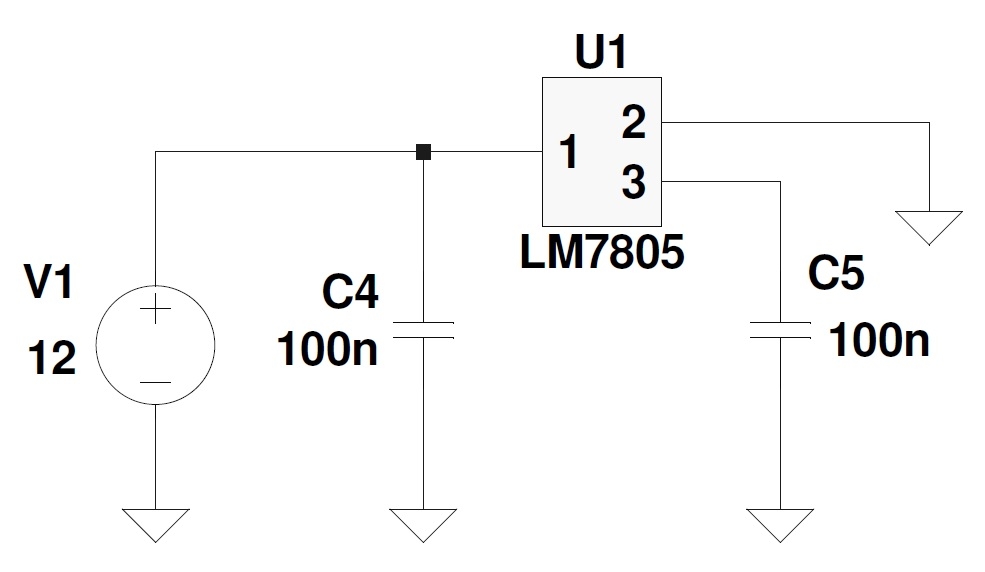
\includegraphics[width = 0.45\linewidth]{Figures/linearreg.jpg}
    \caption{Circuit schematic of the 5V regulator}
    \label{fig:5vregulator}
\end{figure}

\section{Simulation} \label{sec:simulation_linear}
In order to see if the designed circuit operated as required it was simulated in SPICE. The circuit was tested over a various range of load resistor values to see how much power was being consumed and to see if the output voltage remained stable.\newline
These results were listed in Table \ref{tab:linearregtable}, and as can be seen in the last column the power dissipated by the linear regulator was much higher than initially calculated. However this is not a problem as the maximum load requirements do not exceed the maximum power ratings of the linear regulator, and the regulator does not get hot enough to require a heat sink.

\begin{table}
        \centering
        \footnotesize
        \caption{Table showing simulated power consumption of linear regulator.}
         \begin{tabular}{c@{\qquad}rrrr}
          \toprule
           Load Resistance ($\Omega$) & Output Voltage ($\SI{}{V}$) & Power ($\SI{}{\milli W}$) \\
           \midrule
            No load     & 5.0028     & 60.80  \\
            1k          & 5.0028     & 95.72  \\
            470         & 5.0028     & 135.18  \\
            280         & 5.0028     & 185.70 \\
            Full load (125) & 5.0028 & 340.8 \\
          \bottomrule
        \end{tabular}
     \label{tab:linearregtable}
\end{table}

\section{Measurements} \label{sec:measurements_linear}
The measured output voltage of the regulator was found to be $\SI{5.14}{V}$ under no load conditions, and $\SI{5.12}{V}$ under full load conditions supplying $\SI{40}{\milli A}$ as shown in Figure \ref{subfig:5V_reg_output}. This was $2.8\%$ higher than was designed for but still within a acceptable $5\%$ tolerance. As can be seen in Figure \ref{subfig:5V_reg_noise} a noise level of less than $\SI{10}{\milli V}$ peak to peak was measured on the $\SI{5}{V}$ rail, which confirms that the regulator meets all the required specifications. \newline
Furthermore from \cite{reg78L05:2002} it was found that the regulator had a maximum quiescent current of $\SI{5.5}{\milli A}$, given this and a load of $\SI{120}{\Omega}$ the expected efficiency of the regulator was calculated as $37.3\%$ using Equation \ref{eq:efficiency}.

\begin{equation}
   \eta = \frac{P_{out}}{P_{in}}
   \label{eq:efficiency}
\end{equation}

\begin{figure}
 \centering
     \begin{subfigure}[]{0.45\textwidth}
        \centering
         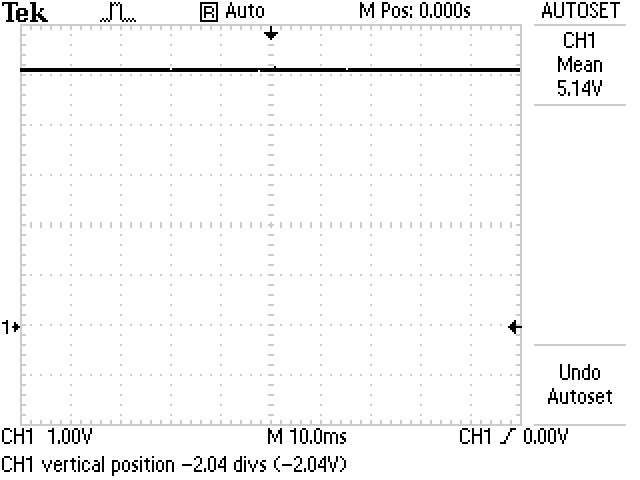
\includegraphics[width=1\linewidth]{./Figures/5V_output_voltage.JPG}
		    \caption{Linear regulator output} \label{subfig:5V_reg_output}
     \end{subfigure}
      \begin{subfigure}[]{0.45\textwidth}
              \centering
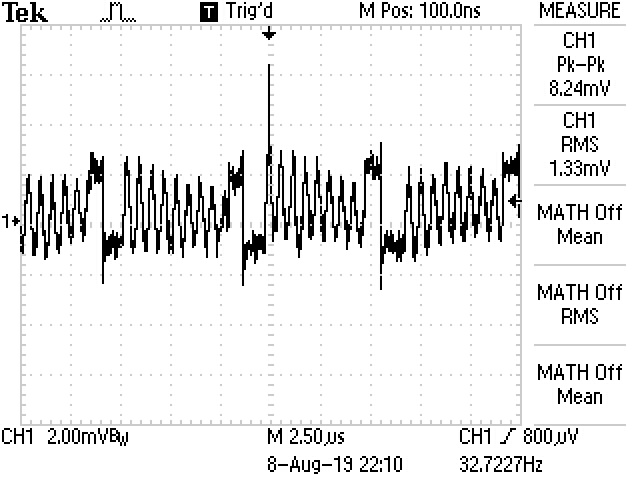
\includegraphics[width=1\linewidth]{./Figures/5V_output_noise.JPG}%
		    \caption{Noise characteristics}  \label{subfig:5V_reg_noise}
     \end{subfigure}
   \caption[Measured 5V Regulated Output Voltage Plots]{Measured 5V Regulated Output Voltage Plots. (a) reading showing output voltage, (b) output noise of the regulator}
    \label{fig:regulator_simulation_results_box}
 \end{figure}








\chapter{System test results}
The signal conditioning system was implemented successfully as can be seen in Figure \ref{fig:system_picture}, all of the sub circuits were tested under various circumstances and passed all of the design requirements with minimal noise interferance. A system test summary can be seen in Table \ref{tab:powersupplytable} showing the total current supplied by the respective power supplies to the signal conditioning circuitry, as well as the voltage level of these power supplies.

\begin{figure}
    \centering
    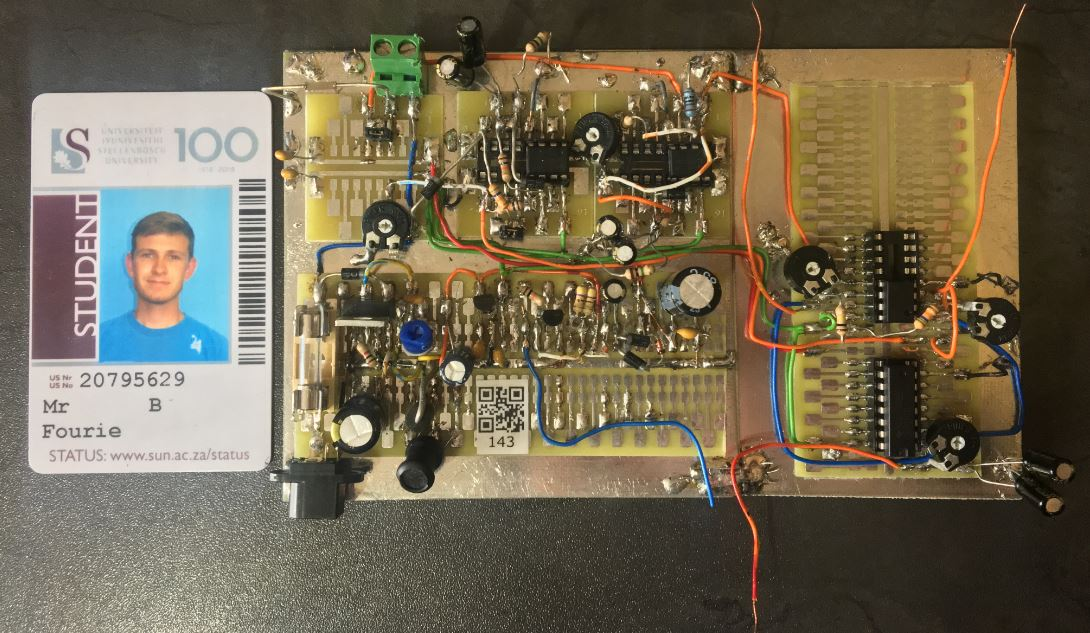
\includegraphics[width = 0.6\linewidth]{Figures/system_picture.JPG}
    \caption{Signal Conditioning Circuitry}
    \label{fig:system_picture}
\end{figure}

\begin{table}
        \centering
        \footnotesize
        \caption{Table showing system test summary.}
         \begin{tabular}{|C{2.5cm}|C{2cm}|C{2.7cm}|C{2.7cm}|}
          \hline
           Regulator & Rail Voltage ($\SI{}{V_{peak}}$) &  Current Supplied ($\SI{}{mA_{peak}}$) & Measured Noise ($\SI{}{mV_{peak}}$) \\
           \hline
           $\SI{5}{V}$ regulator    & 5.04    & 22.09    & 4.71   \\
           $\SI{-5}{V}$ regulator   & -5.12   &  0  & 3.53  \\
          \hline
        \end{tabular}
     \label{tab:powersupplytable}
\end{table}















\appendix%===========================================================


\backmatter%=========================================================

\bibliography{References}
\renewcommand{\thesection}{A.\arabic{section}}
\renewcommand{\thechapter}{A.}
\begin{appendix}

     \chapter{Appendix A: GitHub activity heatmap}

     \begin{figure}[!htb]
     \centering
     	\fbox{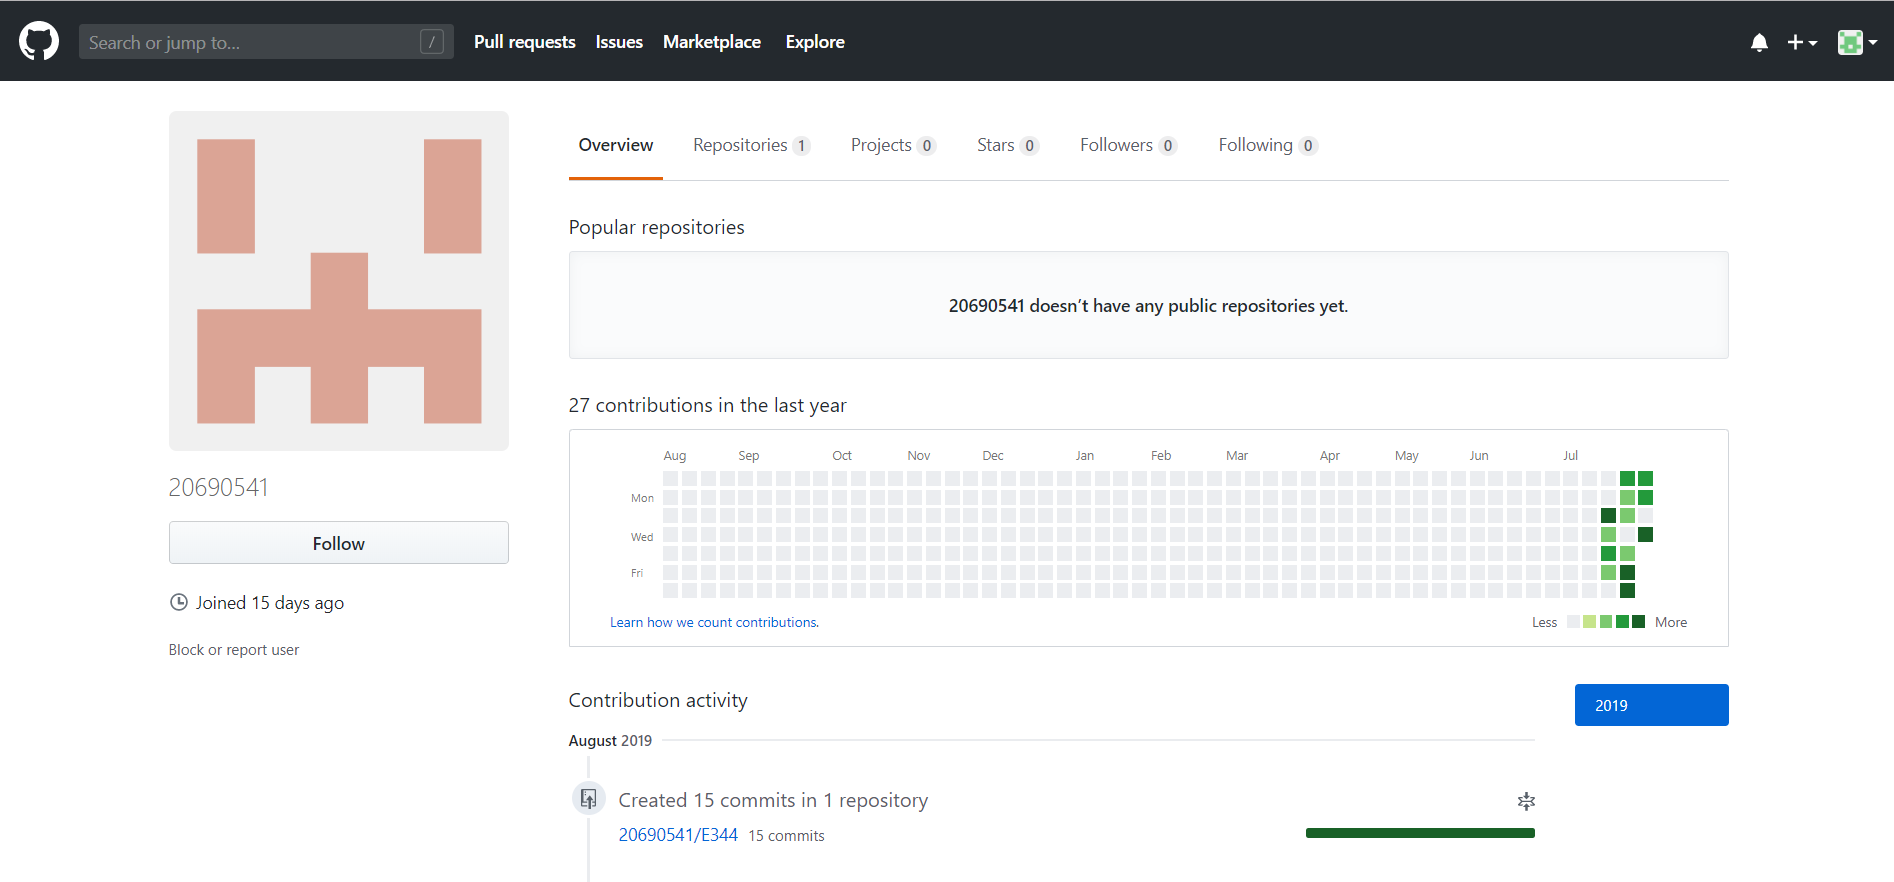
\includegraphics[width=1\linewidth]{./Figures/GitHub.png}}
	\label{fig:github}
	\end{figure}
     \chapter{Appendix B: Wiring safety check}
     \vspace{-15mm}
     \begin{figure}[!htb]
     \centering
     	\fbox{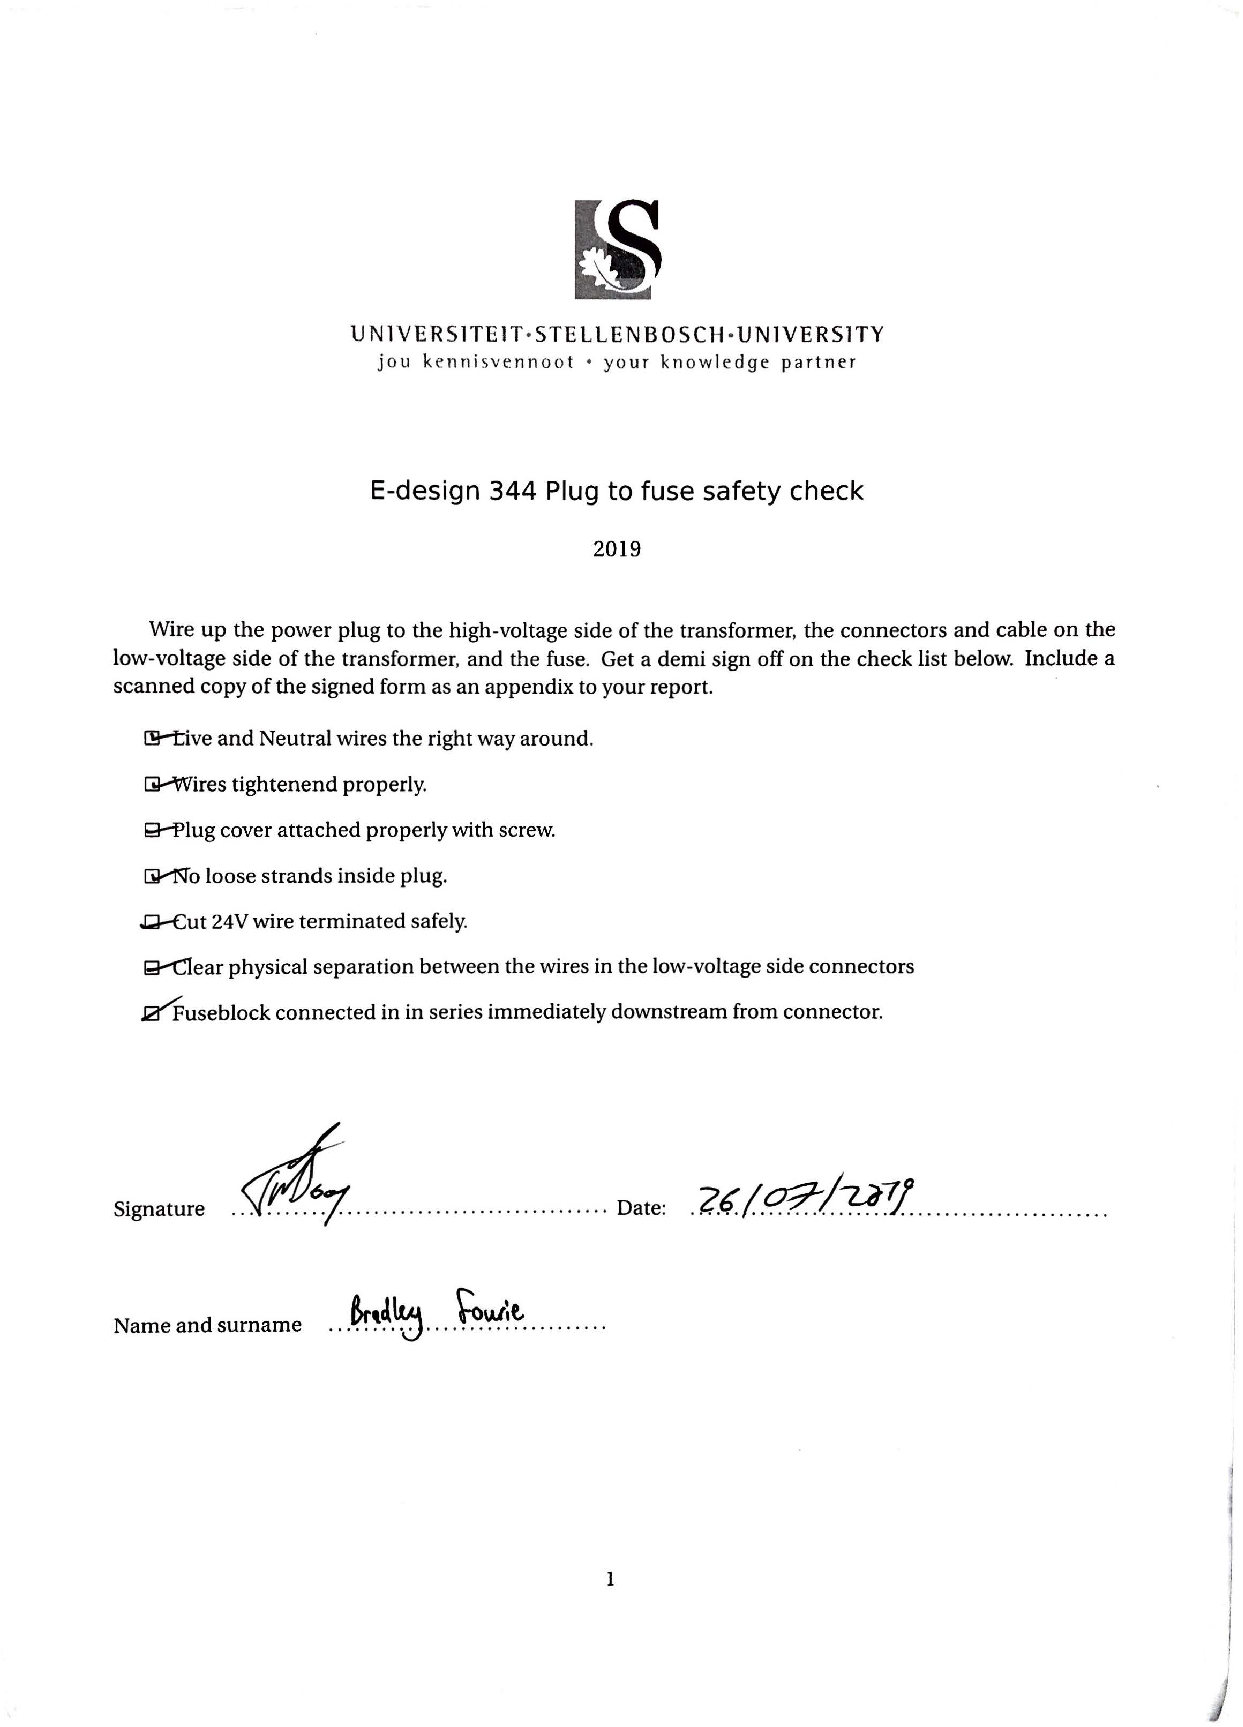
\includegraphics[width=0.78\linewidth]{./Figures/PlugSafetyCheck.pdf}}
	\label{fig:plugSafety}
	\end{figure}
\chapter{Appendix C: Communication protocol between the Beetle and GUI}

\begin{table} [h!]
        \centering
        \footnotesize
        \caption{Communication protocol commands from PC to Beetle}
         \begin{tabular}{C{4cm} C{4cm} C{2cm} C{4cm}}
           Command & Response & First Byte & Second Byte\\
        \hline
            Request Uptime & Requests a string displaying runtime in HH:mm:ss format & 'U' & None \\
            Debug Mode & Requests student number and all the port readings in a comma seperate format  & 'X' & 0-disable \& 1-enable \\
            Request Student Number & Requests student number & '0' & None \\
            Request Analogue Reading & Requests analogue pin reading as a number in bits for debugging purposes & '1' & 0-Phase \& 1-Current \& 2-Voltage  \\
            Request Digital Reading & Requests digital pin input/output status for debugging purposes & '2' & 0-Charge pump signal \& 1-SR latch output \& 2-Reset  \\
            Request Trip Reset & Requests digital pin for reset to go high & 'T' & None  \\
          \hline
        \end{tabular}
     \label{tab:commsprotocal1}
\end{table}

\begin{table} [h!]
        \centering
        \footnotesize
        \caption{Communication protocol response from Beetle to PC}
         \begin{tabular}{C{4cm} C{5cm} C{6cm}}
           Command & Response & Payload\\
        \hline
            Print Uptime & Prints a string displaying runtime in HH:mm:ss format & Uptime string as HH:mm:ss \\
            Debug Mode & Prints student number and all the port readings in a comma seperate format  & Debug string as student number, analogue pins and readings, digital pins and readings\\
            Print Student Number & Prints student number & Student number as 8 characters \\
            Print Analogue Reading & Prints analogue pin reading as a number in bits for debugging purposes & Port number followed by analogue value \\
            Print Digital Reading & Prints digital pin input/output status for debugging purposes & Port number followed by high or low status \\
            Print Routine Measurements & Prints calibrated transducer measurements and trip switch status every second & Phase, current and voltage transducer readings followed by trip switch status\\
          \hline
        \end{tabular}
     \label{tab:commsprotocal2}
\end{table}
\end{appendix}
\end{document}
